    \documentclass[10pt]{beamer}

    \usepackage{stmaryrd}
    \usepackage{beamerthemesplit}
    \usepackage{xcolor}
    \usepackage{hyperref}

    \usepackage[italian]{babel}
  \usepackage[utf8x]{inputenc}

    \newcommand{\TSync}[0]{\ltimes}
    \newcommand{\TWait}[0]{\rtimes}
    \newcommand{\TTot}[0]{\bowtie}


    %\usetheme{Antibes}
    \usetheme{Darmstadt}
    % per trasparenza su animazioni di blocchi
    \setbeamercovered{dynamic}



    \title{Misurare Processi di Business}
    \author{R.Bruni \and A.Corradini  \and G.Ferrari \and
      T.Flagella \and R.Guanciale  \and \alert{G.O.Spagnolo}}
    \date{\today \\ \textbf{\alert{Conferenza AICA 2011} - Torino}}


    \begin{document}

    \frame{\titlepage}

    \section{Introduzione}
    \subsection{Business Process Management}
    \frame{
      \begin{block}{Business Process Management}
	\begin{itemize}
	\item BPM affronta la modellazione, l'organizzazione, l'applicazione e
    l'ottimizzazione delle attivit\`a necessarie per raggiungere un
    determinato obiettivo (es. offrire un determinato servizio, oppure produrre
    un certo manufatto).

    \item In BPM, i processi vengono rappresentati attraverso formalismi grafici,
    permettendo di comunicare in modo non ambiguo le regole di business, 
    e quindi discuterle o modificarle, tra gli svariati ruoli coinvolti  che vanno dagli esperti del dominio di
    business o del settore, agli architetti software e sviluppatori.
	\end{itemize}
      \end{block}
    }

    \subsection{Sommario}
    \frame{
      \begin{block}{Obiettivi}
	\begin{itemize}
      
	\item In questo contributo ci focalizziamo su una specifica fase del BPM, che comprende
  il monitoraggio e la valutazione. L’obiettivo di questa fase consiste nel
  verificare la corretta esecuzione dei processi e misurarne le prestazioni dopo il
  loro deployment.
	\end{itemize}
      \end{block}
      \begin{block}{Strategia}
	\begin{itemize}
	\item Adottare ed estendere esistenti metodi formali (Petri Nets)
	\item Integrare ed estendere esistenti infrastutture software (ProM)
	\item Metodologia dei work-flow
	  \begin{enumerate}
	  \item I processi sono descritti con BPMN diagrams
	  \item Il BPMN diagram viene trasformato in una Petri Net
	  \item I log delle istanze di processo sono processati usando tecniche disponibili per le Petri Net
	  \item I risultati delle analisi sono proiettati indietro sul modello di partenza BPMN.
	  \end{enumerate}
	\end{itemize}

      \end{block}
    }

    \section{Supporto alla modellazione tramite BPMN}
    \subsection{From BPMN to Petri Net}
  %   \frame{
  %     \begin{block}{Esempio di modello BPMN}
  %       \begin{itemize}
  % 	\item Permette di modellare i processi ad un alto livello di astrazione, questo modello può essere compreso o creato anche
  %   dai non addetti ai lavori.
  %       \end{itemize}
  %     \end{block}
  %     
  %     \begin{center}
  %       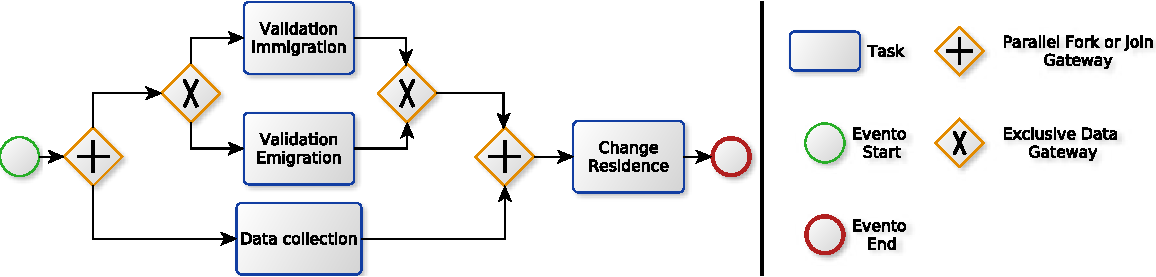
\includegraphics[scale=0.50]{./fig/residency2}
  %     \end{center}
  % 
  %   }

    \frame{
      \begin{block}{From BPMN to Petri Net}
	\begin{itemize}
	  \item Sfruttiamo una metodologia di trasformazione esistente (Dijkman, R.M., Dumas, M., Ouyang, C.) estesa
	  \item Successivamente affrontiamo il problema di
    riportare i risultati di queste analisi sul modello BPMN di partenza.
	\end{itemize}
      \end{block}
      
      \begin{center}
	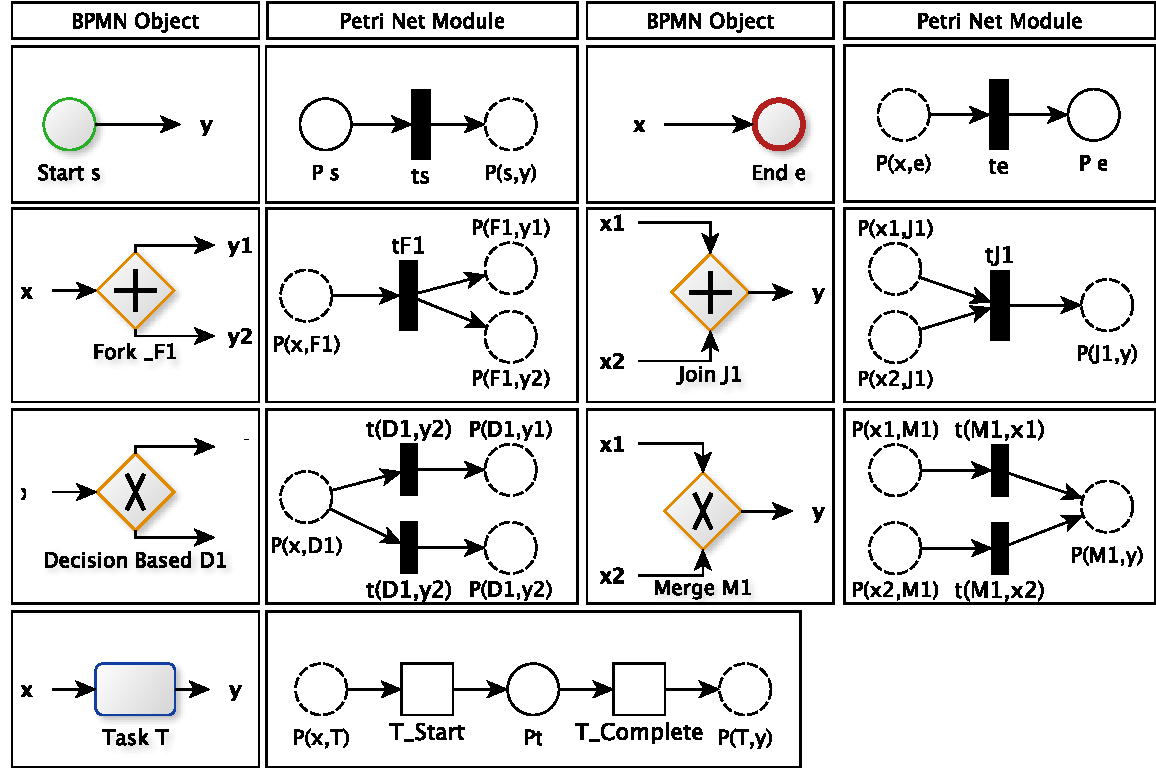
\includegraphics[scale=0.30]{./fig/MappingBPMNtoPN}
      \end{center}

    }
  %  \frame{
  %       
  % 	\begin{center}
  % 	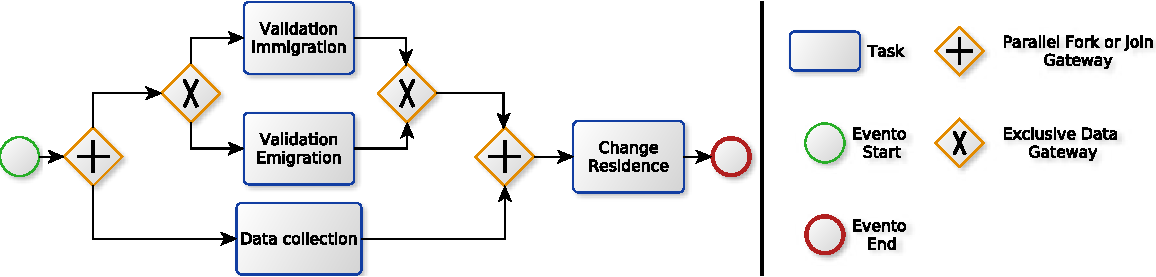
\includegraphics[scale=0.5]{./fig/residency2}
  %       \end{center}
  %       
  %       
  %       \begin{center}
  % 	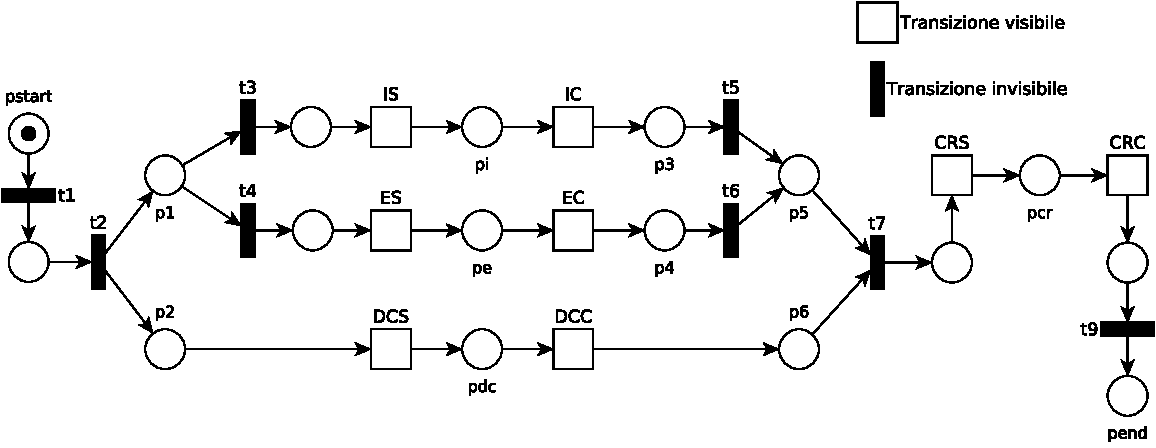
\includegraphics[scale=0.5]{./fig/residencyPN}
  %       \end{center}
  % 
  %     }


    \frame{
	
	  \begin{center}
	  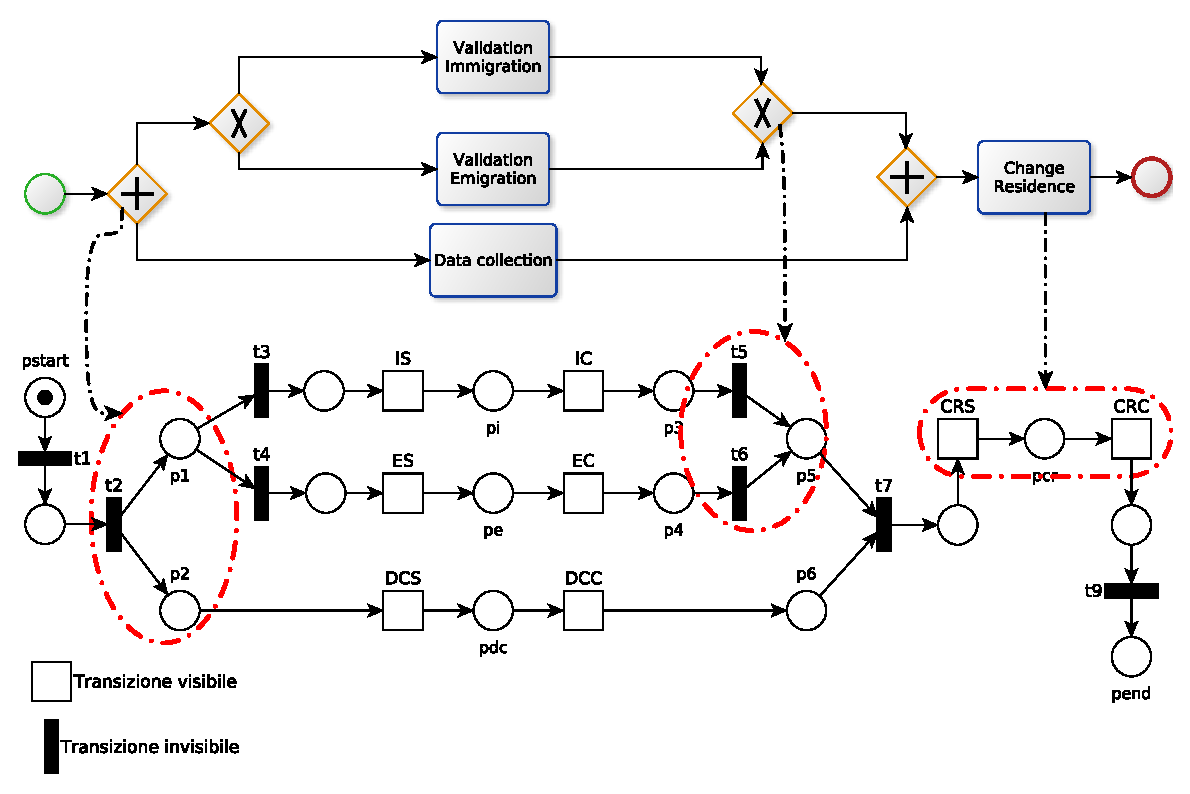
\includegraphics[scale=0.6]{./fig/residencyPN33}
	\end{center}
	
	


      }


    \section{Analisi basata su Petri Nets}
    \subsection{Analisi basata su Petri Nets}
    \frame{
      \begin{block}{Analisi basata su Petri Nets}
	
	\begin{itemize}
	  \item Gli eventi delle istanze di processo del log sono ordinati
	    (e.s. timestamp)
	  \item Gli eventi sono mappati sulle transizioni della rete
	  \item \alert{Log Replay}: replay delle istanze di processo del log
	    (non-blocking way)
	    
	    \begin{enumerate}
	    % \item Put a token in the start place
	      \item L'algoritmo parte con un token nella piazza iniziale
    delle rete
	      \item Estrae dalla testa del log l'evento
	      \item Viene effettuato il fire della corrispondente transizione
		\begin{itemize}
		  \item Se la transizione non è abilitata i token
    mancanti vengono creati artificialmente e chiamati \textbf{missing token}
		\end{itemize}
	    \end{enumerate}
	  \item Metriche
	    \begin{itemize}
	      \item Il numero di missing/remaining token per ogni piazza/transizione
	      \item Il numero di archi attraversati
	      \item Il tempo di soggiorno/attesa/sincronizzazione per ogni piazza.
	    \end{itemize}
	\end{itemize}

      \end{block}
    }

  % \frame{
  \begin{block}{Log-replay examples}
    Trace log $(A, 1s), (B, 2s), (C, 4s), (D, 8s)$ 
  \end{block}
  \begin{center}
    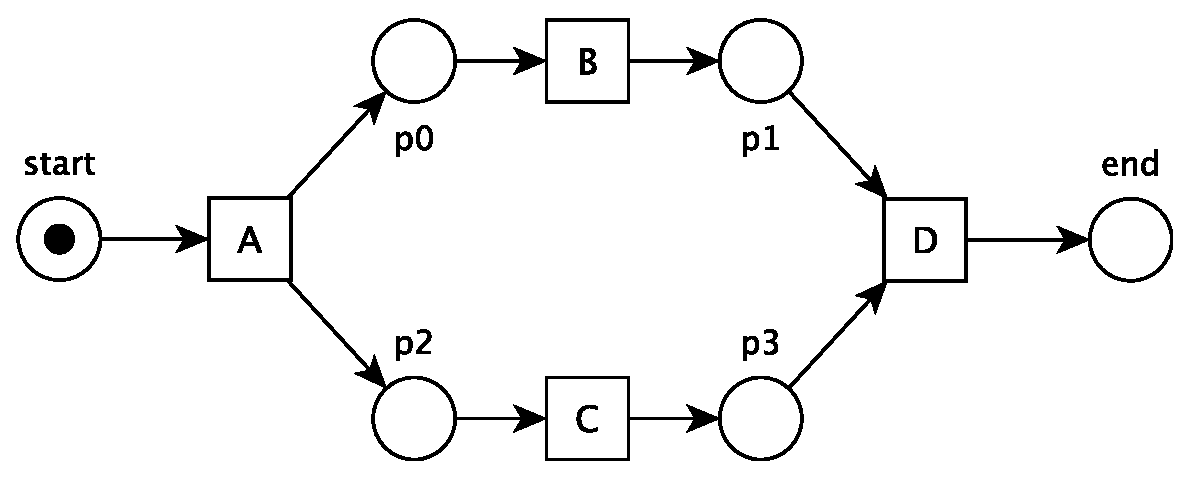
\includegraphics[scale=0.30]{./fig/LogReplay1a}
  \end{center}
  \begin {block}{Measures}
    \begin{tabular}{cc}
    \end{tabular}
  \end{block}
}
\frame{
  \begin{block}{Log-replay examples}
    Trace log $\alert{(A, 1s)}, (B, 2s), (C, 4s), (D, 8s)$ 
  \end{block}
  \begin{center}
    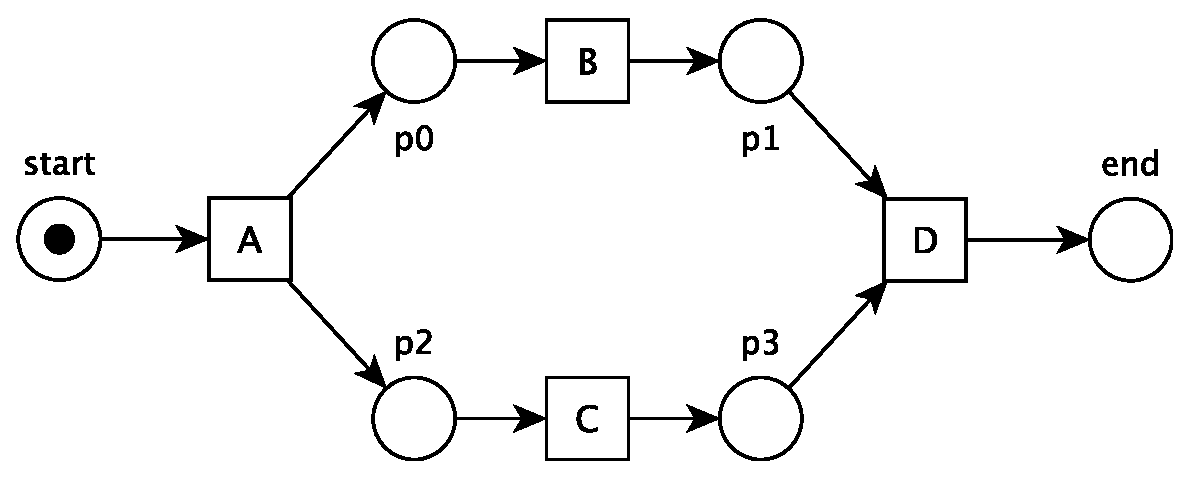
\includegraphics[scale=0.30]{./fig/LogReplay1a}
  \end{center}
  \begin {block}{Measures}
    \begin{tabular}{cc}
    \end{tabular}
  \end{block}
}
\frame{
  \begin{block}{Log-replay examples}
    Trace log $\alert{(A, 1s)}, (B, 2s), (C, 4s), (D, 8s)$ 
  \end{block}
  \begin{center}
    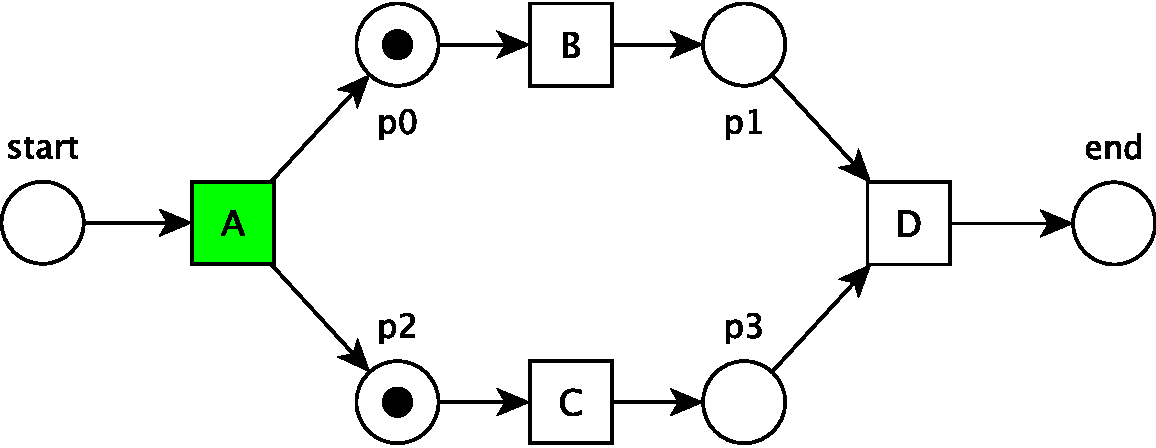
\includegraphics[scale=0.30]{./fig/LogReplay1b}
  \end{center}
  \begin {block}{Measures}
    \begin{tabular}{ccc}
                  & p0 & p2 \\
       $\TSync$   & 0  & 0  \\
    \end{tabular}
  \end{block}
}
\frame{
  \begin{block}{Log-replay examples}
    Trace log $(A, 1s), \alert{(B, 2s)}, (C, 4s), (D, 8s)$ 
  \end{block}
  \begin{center}
    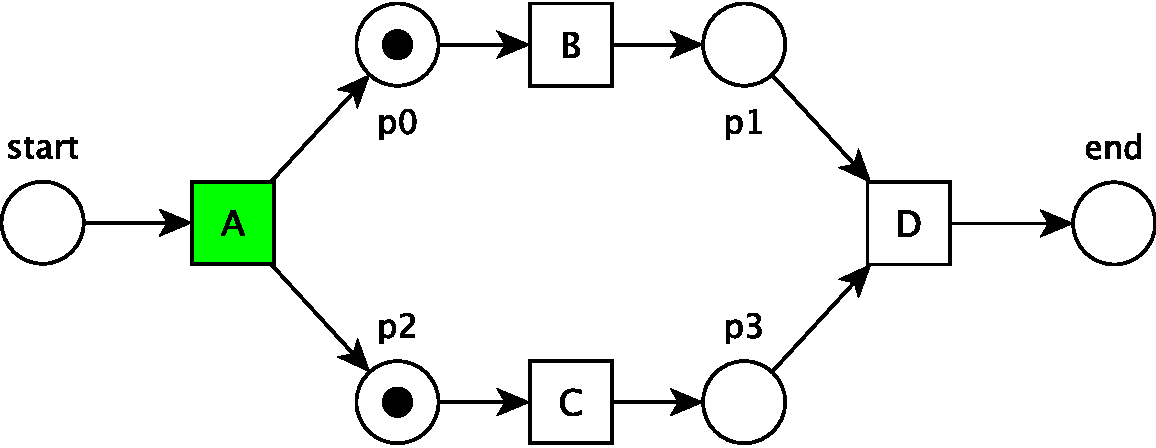
\includegraphics[scale=0.30]{./fig/LogReplay1b}
  \end{center}
  \begin {block}{Measures}
    \begin{tabular}{ccc}
                  & p0 & p2 \\
       $\TSync$   & 0  & 0  \\
    \end{tabular}
  \end{block}
}
\frame{
  \begin{block}{Log-replay examples}
    Trace log $(A, 1s), \alert{(B, 2s)}, (C, 4s), (D, 8s)$ 
  \end{block}
  \begin{center}
    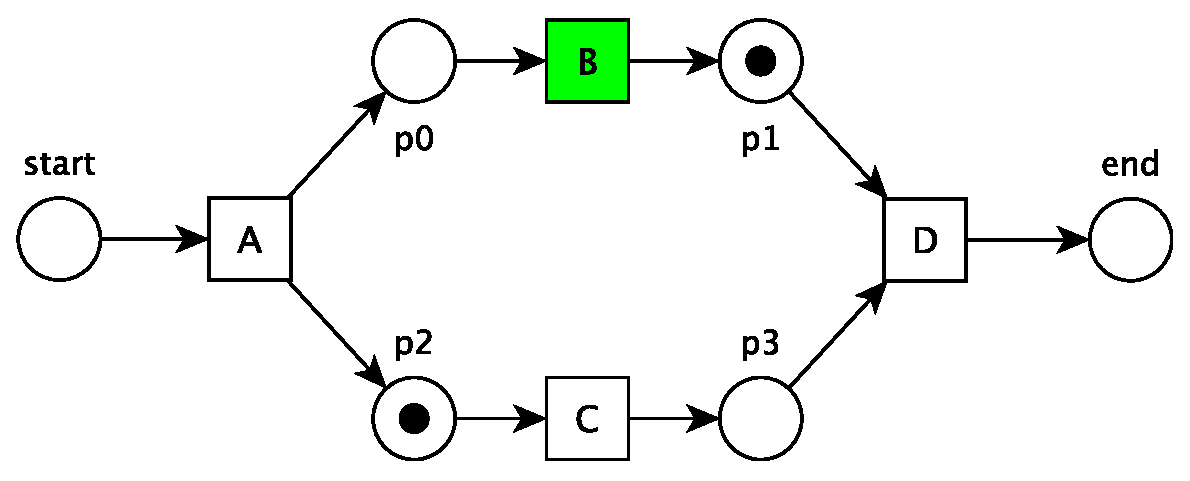
\includegraphics[scale=0.30]{./fig/LogReplay1c}
  \end{center}
  \begin {block}{Measures}
    \begin{tabular}{ccc}
                  & p0 & p2 \\
       $\TSync$   & 0  & 0  \\
       $\TTot$    & 1  &    \\
    \end{tabular}
  \end{block}
}
\frame{
  \begin{block}{Log-replay examples}
    Trace log $(A, 1s), (B, 2s), \alert{(C, 4s)}, (D, 8s)$ 
  \end{block}
  \begin{center}
    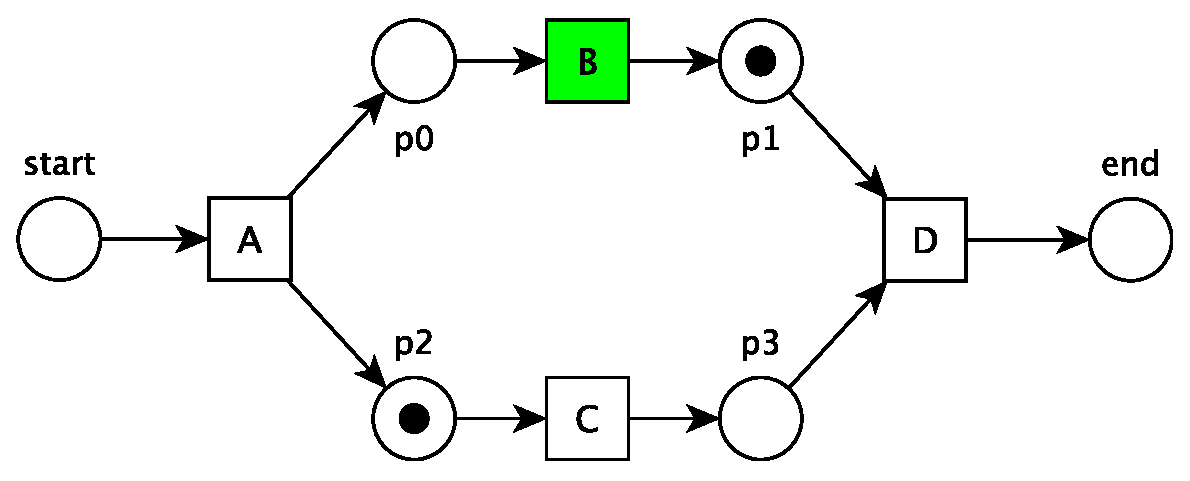
\includegraphics[scale=0.30]{./fig/LogReplay1c}
  \end{center}
  \begin {block}{Measures}
    \begin{tabular}{ccc}
                  & p0 & p2 \\
       $\TSync$   & 0  & 0  \\
       $\TTot$    & 1  &    \\
    \end{tabular}
  \end{block}
}
\frame{
  \begin{block}{Log-replay examples}
    Trace log $(A, 1s), (B, 2s), \alert{(C, 4s)}, (D, 8s)$ 
  \end{block}
  \begin{center}
    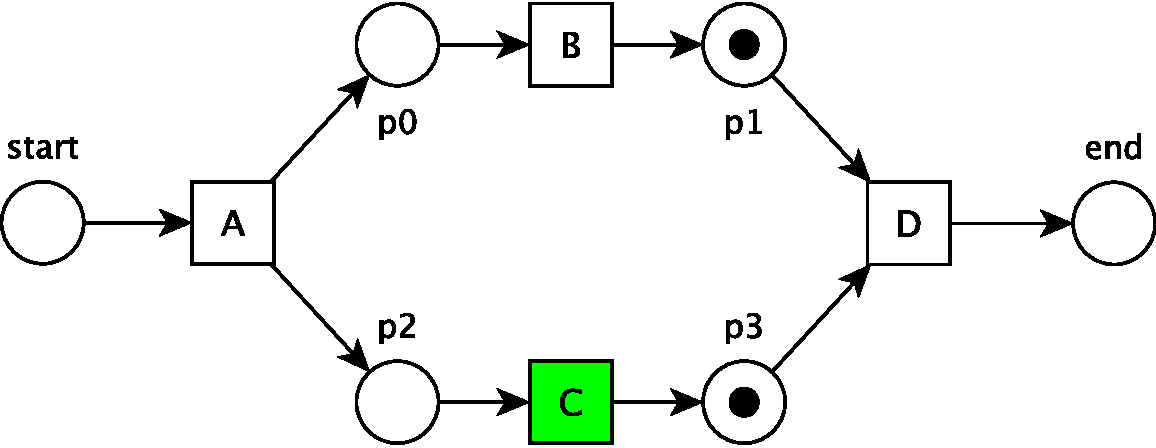
\includegraphics[scale=0.30]{./fig/LogReplay1d}
  \end{center}
  \begin {block}{Measures}
    \begin{tabular}{ccccccccc}
                  & p0 & p2 & p1 & p3 \\
       $\TSync$   & 0  & 0  & 2  & 0  \\
       $\TTot$    & 1  & 3  &    &    \\
    \end{tabular}
  \end{block}
}
\frame{
  \begin{block}{Log-replay examples}
    Trace log $(A, 1s), (B, 2s), (C, 4s), \alert{(D, 8s)}$ 
  \end{block}
  \begin{center}
    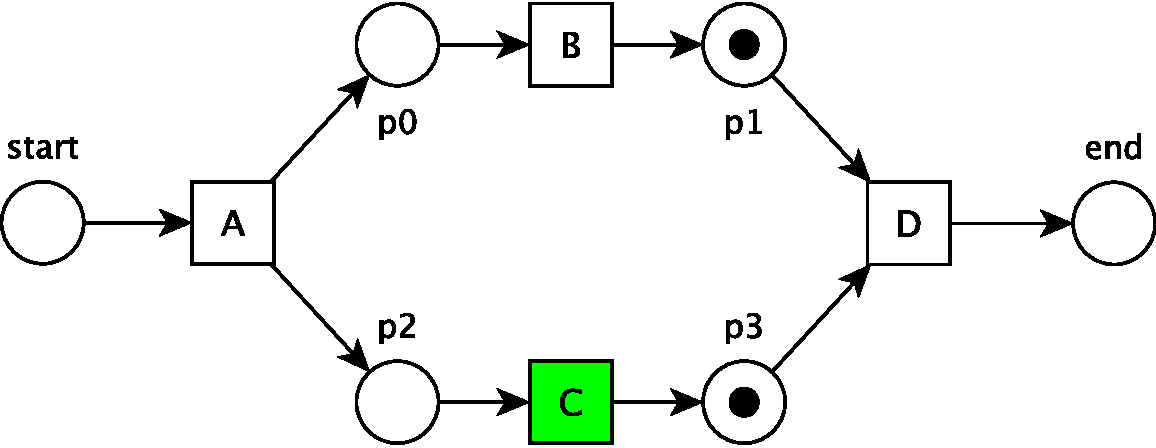
\includegraphics[scale=0.30]{./fig/LogReplay1d}
  \end{center}
  \begin {block}{Measures}
    \begin{tabular}{ccccccccc}
                  & p0 & p2 & p1 & p3 \\
       $\TSync$   & 0  & 0  & 2  & 0  \\
       $\TTot$    & 1  & 3  &    &    \\
    \end{tabular}
  \end{block}
}
\frame{
  \begin{block}{Log-replay examples}
    Trace log $(A, 1s), (B, 2s), (C, 4s), \alert{(D, 8s)}$ 
  \end{block}
  \begin{center}
    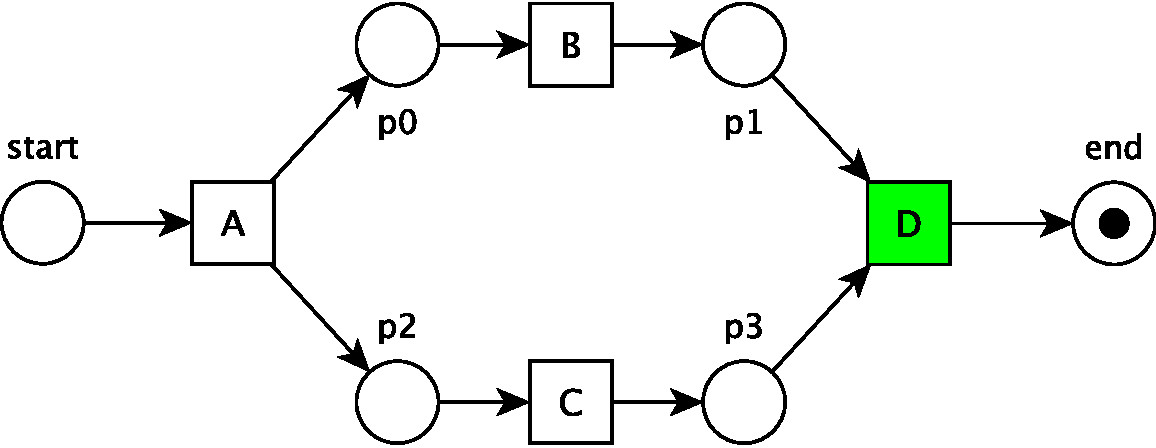
\includegraphics[scale=0.30]{./fig/LogReplay1e}
  \end{center}
  \begin {block}{Measures}
    \begin{tabular}{ccccccccc}
                  & p0 & p2 & p1 & p3 \\
       $\TSync$   & 0  & 0  & 2  & 0  \\
       $\TTot$    & 1  & 3  & 6  & 4  \\
    \end{tabular}
  \end{block}
}

%%% Local Variables: 
%%% mode: latex
%%% TeX-master: "main"
%%% End: 

  % \frame{
  \begin{block}{Log-replay examples}
    Trace log $(A, 1s), (B, 2s), (D, 8s)$ 
  \end{block}
  \begin{center}
    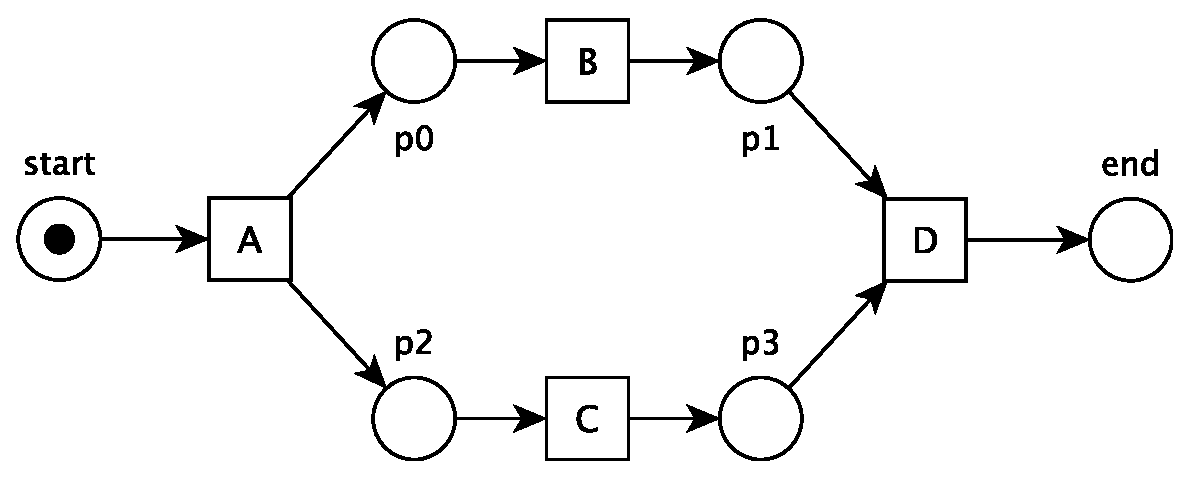
\includegraphics[scale=0.30]{./fig/LogReplay1a}
  \end{center}
  \begin {block}{Measures}
    \begin{tabular}{cc}
    \end{tabular}
  \end{block}
}
\frame{
  \begin{block}{Log-replay examples}
    Trace log $\alert{(A, 1s)}, (B, 2s), (D, 8s)$ 
  \end{block}
  \begin{center}
    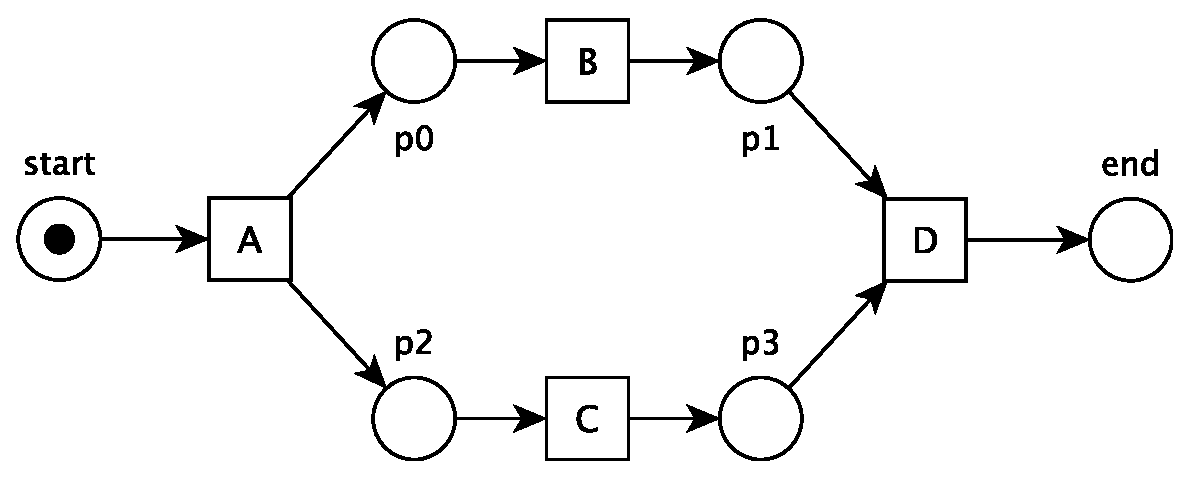
\includegraphics[scale=0.30]{./fig/LogReplay1a}
  \end{center}
  \begin {block}{Measures}
    \begin{tabular}{cc}
    \end{tabular}
  \end{block}
}
\frame{
  \begin{block}{Log-replay examples}
    Trace log $\alert{(A, 1s)}, (B, 2s), (D, 8s)$ 
  \end{block}
  \begin{center}
    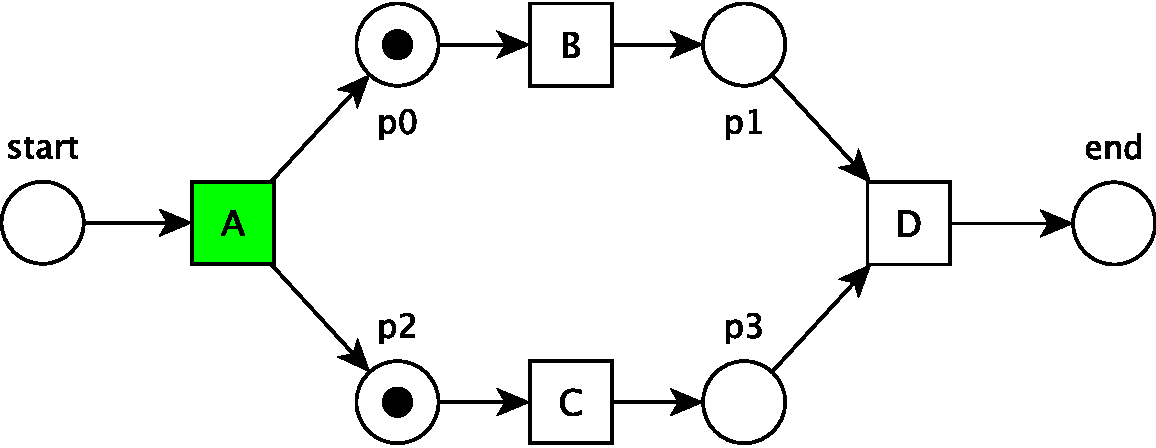
\includegraphics[scale=0.30]{./fig/LogReplay1b}
  \end{center}
  \begin {block}{Measures}
    \begin{tabular}{ccc}
                  & p0 & p2 \\
       $\TSync$   & 0  & 0  \\
    \end{tabular}
  \end{block}
}
\frame{
  \begin{block}{Log-replay examples}
    Trace log $(A, 1s), \alert{(B, 2s)}, (D, 8s)$ 
  \end{block}
  \begin{center}
    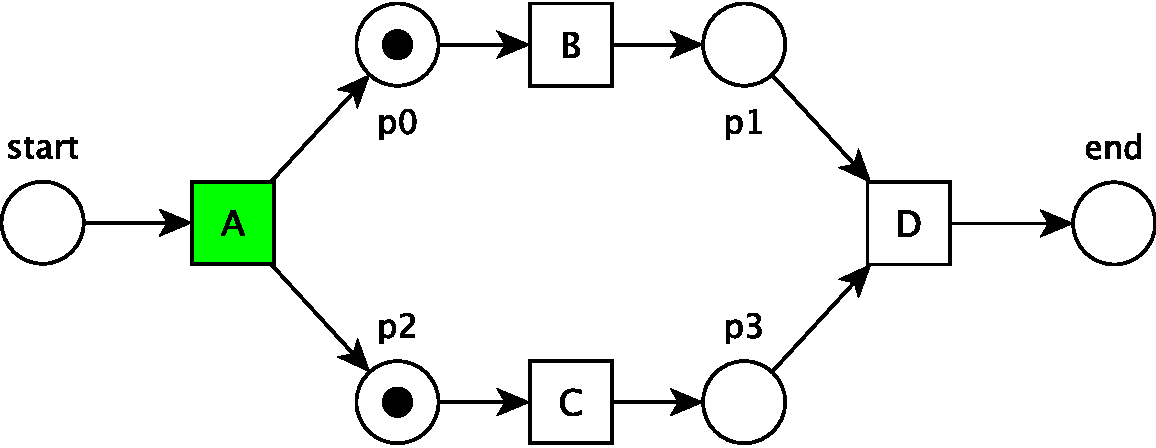
\includegraphics[scale=0.30]{./fig/LogReplay1b}
  \end{center}
  \begin {block}{Measures}
    \begin{tabular}{ccc}
                  & p0 & p2 \\
       $\TSync$   & 0  & 0  \\
    \end{tabular}
  \end{block}
}
\frame{
  \begin{block}{Log-replay examples}
    Trace log $(A, 1s), \alert{(B, 2s)}, (D, 8s)$ 
  \end{block}
  \begin{center}
    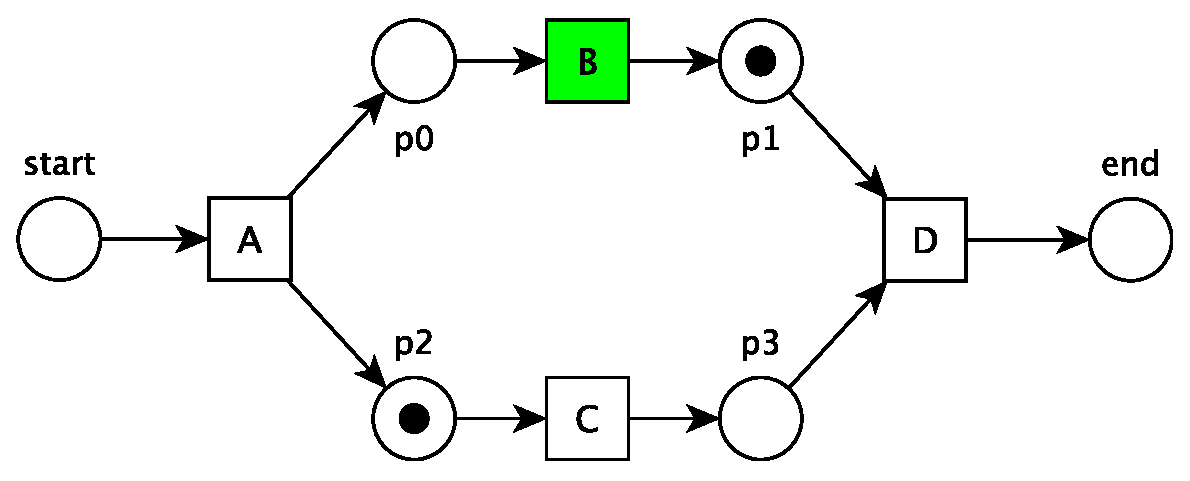
\includegraphics[scale=0.30]{./fig/LogReplay1c}
  \end{center}
  \begin {block}{Measures}
    \begin{tabular}{ccc}
                  & p0 & p2 \\
       $\TSync$   & 0  & 0  \\
       $\TTot$    & 1  &    \\
    \end{tabular}
  \end{block}
}
\frame{
  \begin{block}{Log-replay examples}
    Trace log $(A, 1s), (B, 2s), \alert{(D, 8s)}$ 
  \end{block}
  \begin{center}
    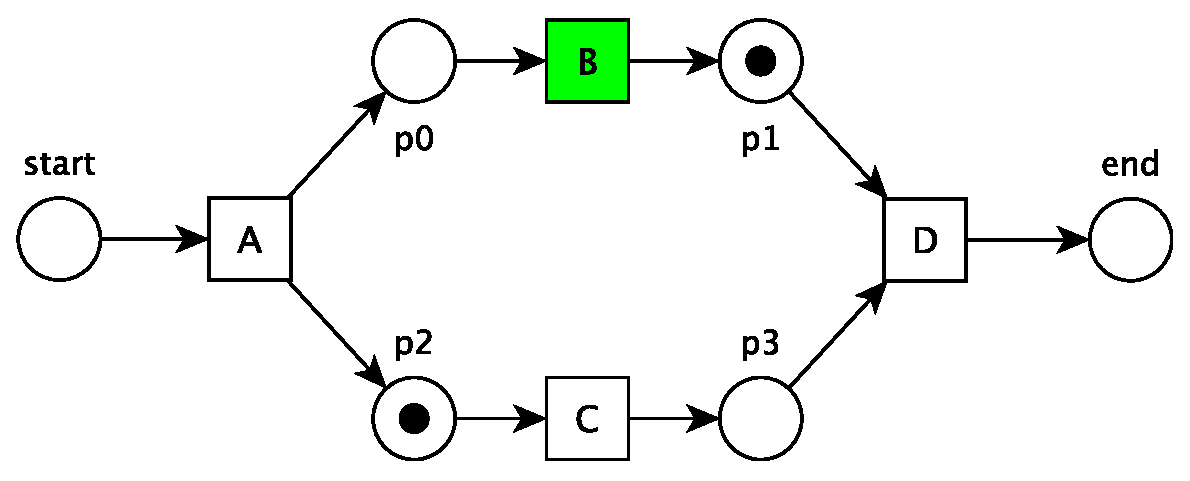
\includegraphics[scale=0.30]{./fig/LogReplay1c}
  \end{center}
  \begin {block}{Measures}
    \begin{tabular}{ccc}
                  & p0 & p2 \\
       $\TSync$   & 0  & 0  \\
       $\TTot$    & 1  &    \\
    \end{tabular}
  \end{block}
}

\frame{
  \begin{block}{Log-replay examples}
    Trace log $(A, 1s), (B, 2s), \alert{(D, 8s)}$ 
  \end{block}
  \begin{center}
    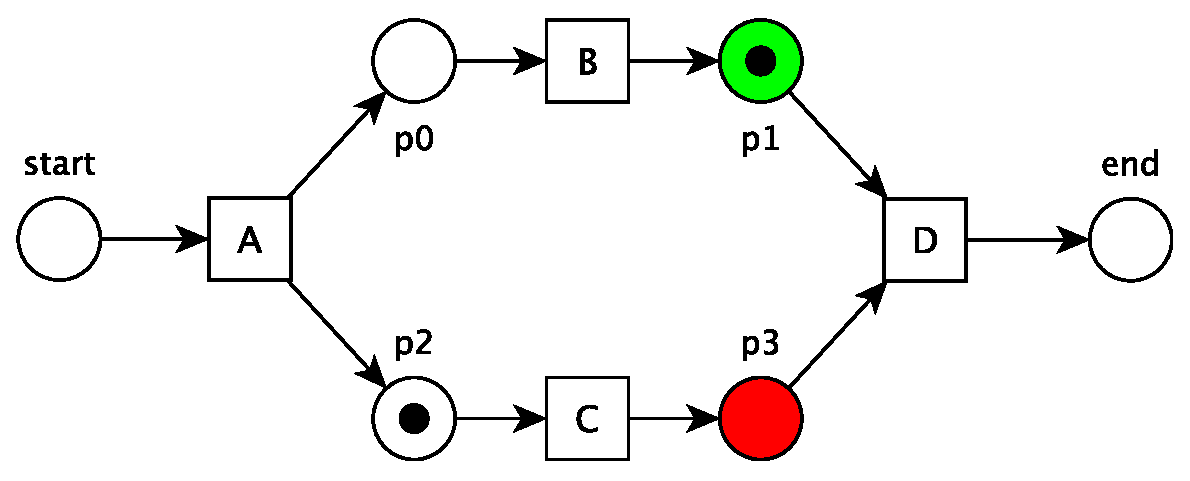
\includegraphics[scale=0.30]{./fig/LogReplay2d}
  \end{center}
  \begin {block}{Measures}
    \begin{tabular}{ccc}
                  & p0 & p2 \\
       $\TSync$   & 0  & 0  \\
       $\TTot$    & 1  &    \\
    \end{tabular}
  \end{block}
}
\frame{
  \begin{block}{Log-replay examples}
    Trace log $(A, 1s), (B, 2s), \alert{(D, 8s)}$ 
  \end{block}
  \begin{center}
    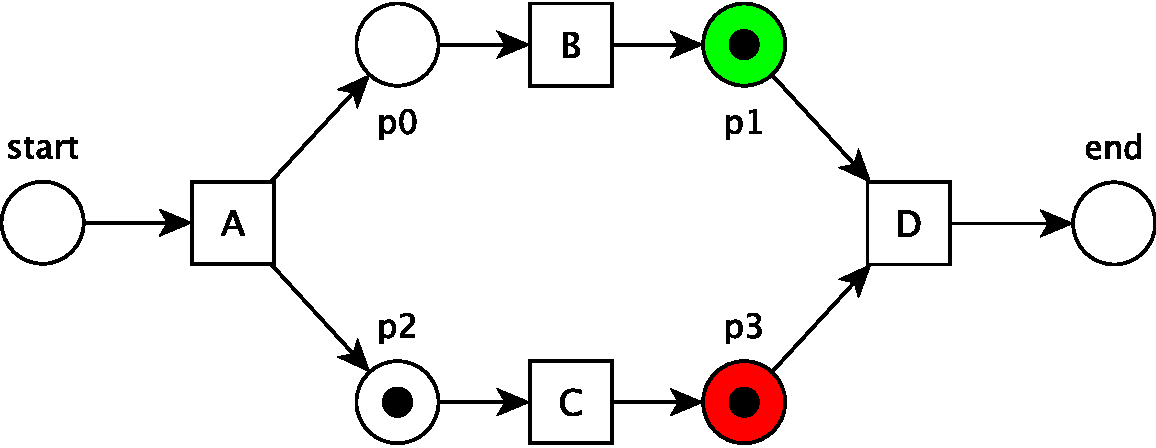
\includegraphics[scale=0.30]{./fig/LogReplay2f}
  \end{center}
  \begin {block}{Measures}
    \begin{tabular}{ccc}
                  & p0 & p2 \\
       $\TSync$   & 0  & 0  \\
       $\TTot$    & 1  &    \\
    \end{tabular}
    \begin{tabular}{ccc}
                  & p3 \\
       $Missing$  & 1  \\
    \end{tabular}
  \end{block}
}
\frame{
  \begin{block}{Log-replay examples}
    Trace log $(A, 1s), (B, 2s), \alert{(D, 8s)}$ 
  \end{block}
  \begin{center}
    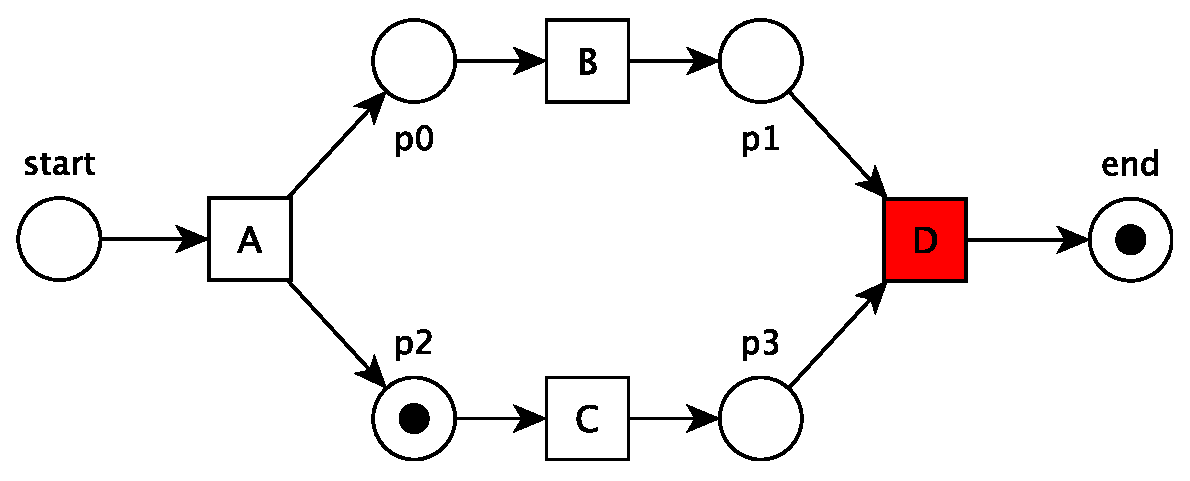
\includegraphics[scale=0.30]{./fig/LogReplay2g}
  \end{center}
  \begin {block}{Measures}
    \begin{tabular}{ccc}
                  & p0 & p2 \\
       $\TSync$   & 0  & 0  \\
       $\TTot$    & 1  &    \\
    \end{tabular}
    \begin{tabular}{ccc}
                  & p3 \\
       $Missing$  & 1  \\
    \end{tabular}
  \end{block}
}
\frame{
  \begin{block}{Log-replay examples}
    Trace log $(A, 1s), (B, 2s), \alert{(D, 8s)}$ 
  \end{block}
  \begin{center}
    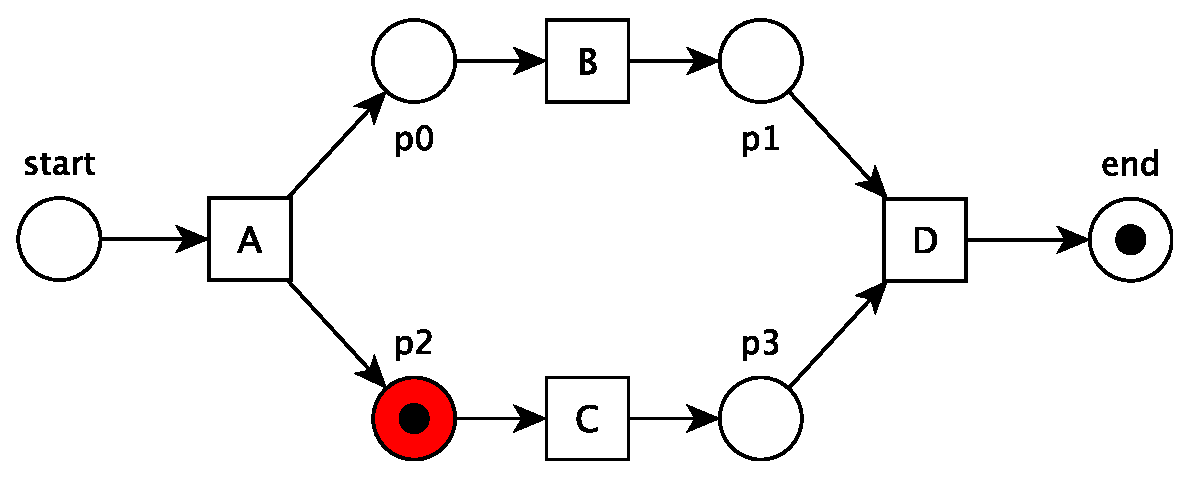
\includegraphics[scale=0.30]{./fig/LogReplay2h}
  \end{center}
  \begin {block}{Measures}
    \begin{tabular}{ccc}
                  & p0 & p2 \\
       $\TSync$   & 0  & 0  \\
       $\TTot$    & 1  &    \\
    \end{tabular}
    \begin{tabular}{ccc}
                   & p3 & p2 \\
       $Missing$   & 1  & 0  \\
       $Remaining$ & 0  & 1   \\
    \end{tabular}
  \end{block}
}


%%% Local Variables: 
%%% mode: latex
%%% TeX-master: "main"
%%% End: 

  % \frame{
  \begin{block}{Log-replay examples}
    Trace log $\alert{(A, 1s)}, (B, 2s), (C, 4), (D, 8s)$ 
  \end{block}
  \begin{center}
    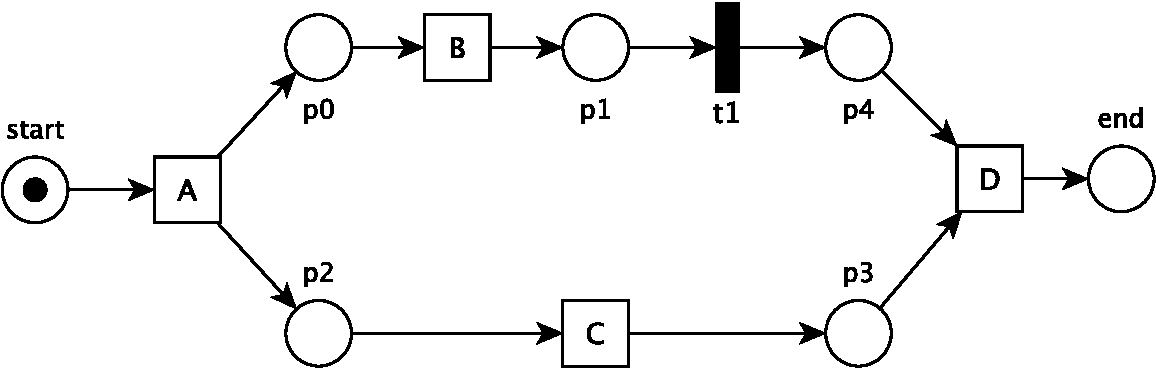
\includegraphics[scale=0.30]{./fig/LogReplay3a}
  \end{center}
  \begin {block}{Measures}
    \begin{tabular}{ccc}
                  \\
       $\TSync$   \\
       $\TTot$    \\
    \end{tabular}
  \end{block}
}
\frame{
  \begin{block}{Log-replay examples}
    Trace log $\alert{(A, 1s)}, (B, 2s), (C, 4), (D, 8s)$ 
  \end{block}
  \begin{center}
    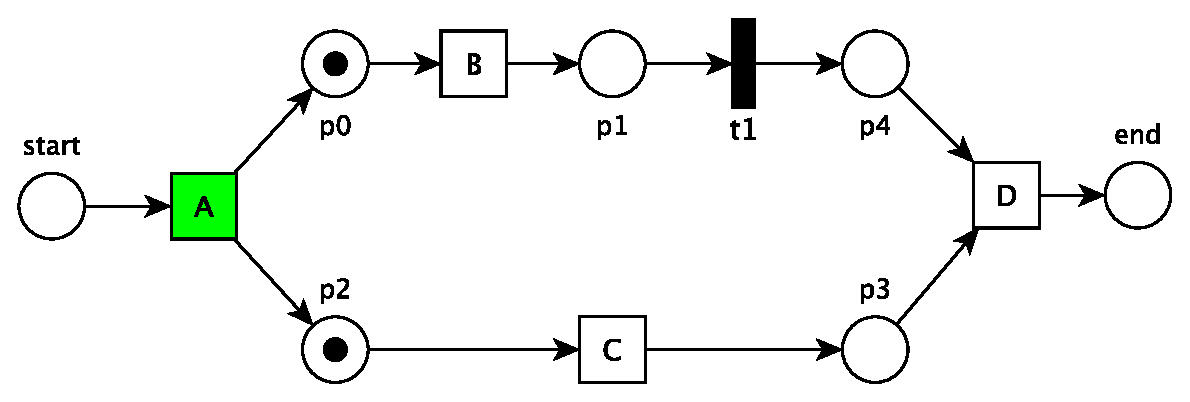
\includegraphics[scale=0.30]{./fig/LogReplay3b}
  \end{center}
  \begin {block}{Measures}
    \begin{tabular}{ccc}
                  & p0 & p2 \\
       $\TSync$   & 0  & 0  \\
       $\TTot$    &    &    \\
    \end{tabular}
  \end{block}
}
\frame{
  \begin{block}{Log-replay examples}
    Trace log $(A, 1s), \alert{(B, 2s)}, (C, 4), (D, 8s)$ 
  \end{block}
  \begin{center}
    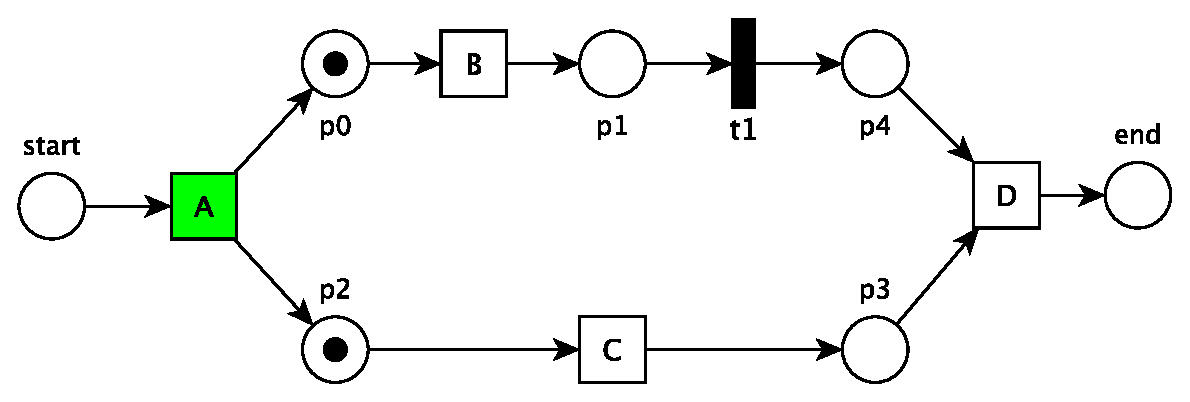
\includegraphics[scale=0.30]{./fig/LogReplay3b}
  \end{center}
  \begin {block}{Measures}
    \begin{tabular}{ccc}
                  & p0 & p2 \\
       $\TSync$   & 0  & 0  \\
       $\TTot$    &    &    \\
    \end{tabular}
  \end{block}
}
\frame{
  \begin{block}{Log-replay examples}
    Trace log $(A, 1s), \alert{(B, 2s)}, (C, 4), (D, 8s)$ 
  \end{block}
  \begin{center}
    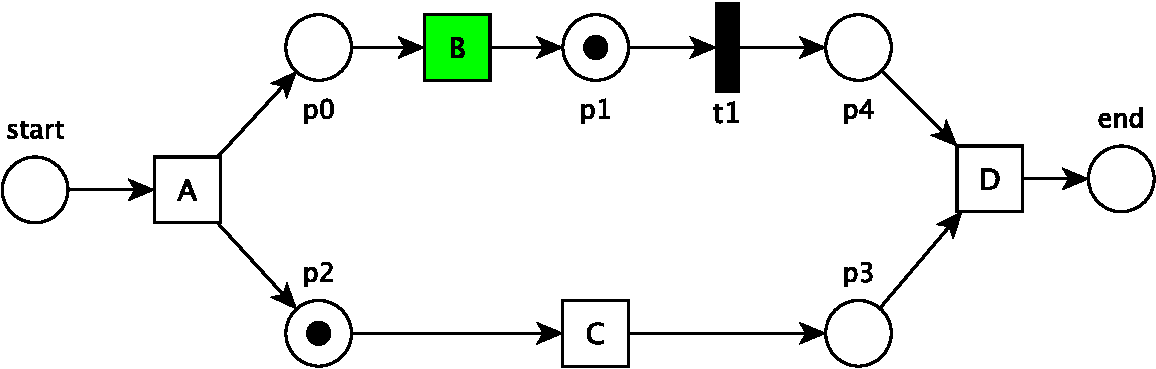
\includegraphics[scale=0.30]{./fig/LogReplay3c}
  \end{center}
  \begin {block}{Measures}
    \begin{tabular}{cccccc}
                  & p0 & p2 & p1 \\
       $\TSync$   & 0  & 0  & 0  \\
       $\TTot$    & 1  &    &    \\
    \end{tabular}
  \end{block}
}

% Attivazione di C
\frame{
  \begin{block}{Log-replay examples}
    Trace log $(A, 1s), (B, 2s), \alert{(C, 4)}, (D, 8s)$ 
  \end{block}
  \begin{center}
    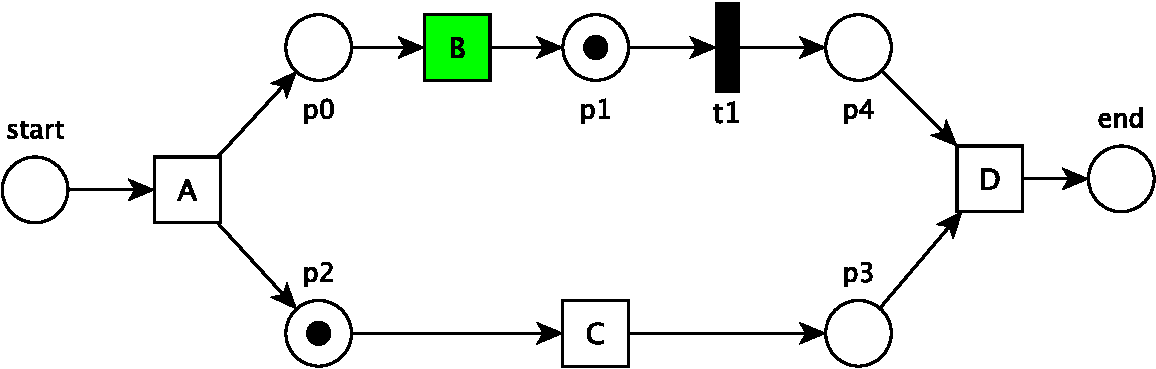
\includegraphics[scale=0.30]{./fig/LogReplay3c}
  \end{center}
  \begin {block}{Measures}
    \begin{tabular}{cccccc}
                  & p0 & p2 & p1 \\
       $\TSync$   & 0  & 0  & 0  \\
       $\TTot$    & 1  &    &    \\
    \end{tabular}
  \end{block}
}
\frame{
  \begin{block}{Log-replay examples}
    Trace log $(A, 1s), (B, 2s), \alert{(C, 4)}, (D, 8s)$ 
  \end{block}
  \begin{center}
    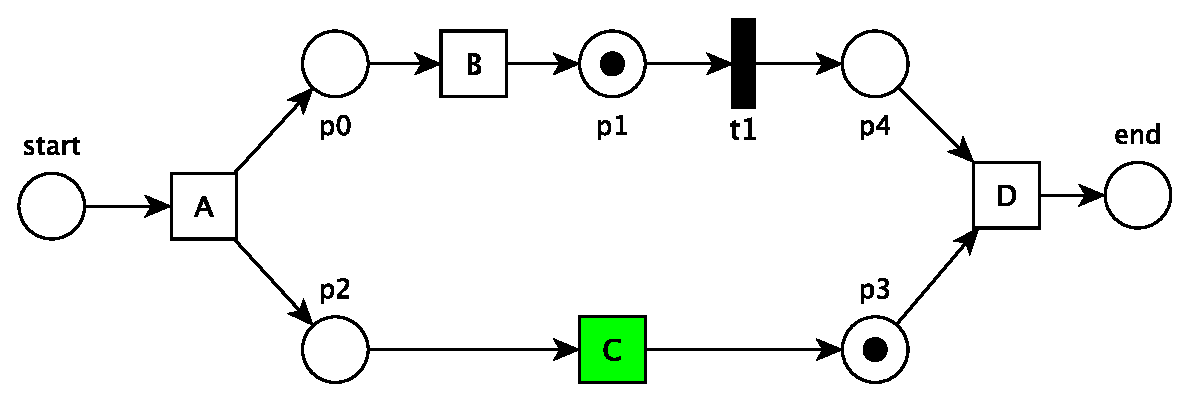
\includegraphics[scale=0.30]{./fig/LogReplay3d}
  \end{center}
  \begin {block}{Measures}
    \begin{tabular}{cccccc}
                  & p0 & p2 & p1 & p3 \\
       $\TSync$   & 0  & 0  & 0  &    \\
       $\TTot$    & 1  & 3  &    &    \\
    \end{tabular}
  \end{block}
}

% attivazione D
\frame{
  \begin{block}{Log-replay examples}
    Trace log $(A, 1s), (B, 2s), (C, 4), \alert{(D, 8s)}$ 
  \end{block}
  \begin{center}
    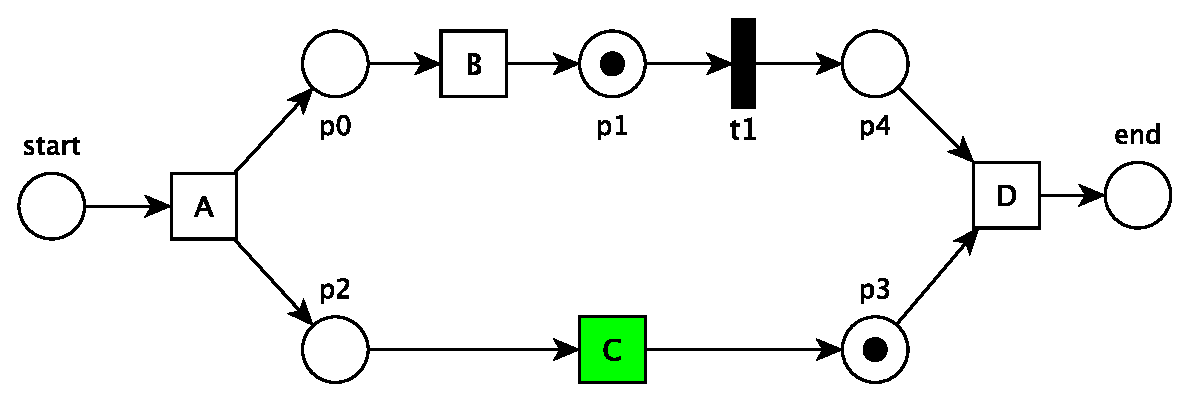
\includegraphics[scale=0.30]{./fig/LogReplay3d}
  \end{center}
  \begin {block}{Measures}
    \begin{tabular}{cccccc}
                  & p0 & p2 & p1 & p3 \\
       $\TSync$   & 0  & 0  & 0  &    \\
       $\TTot$    & 1  & 3  &    &    \\
    \end{tabular}
  \end{block}
}
\frame{
  \begin{block}{Log-replay examples}
    Trace log $(A, 1s), (B, 2s), (C, 4), \alert{(D, 8s)}$ 
  \end{block}
  \begin{center}
    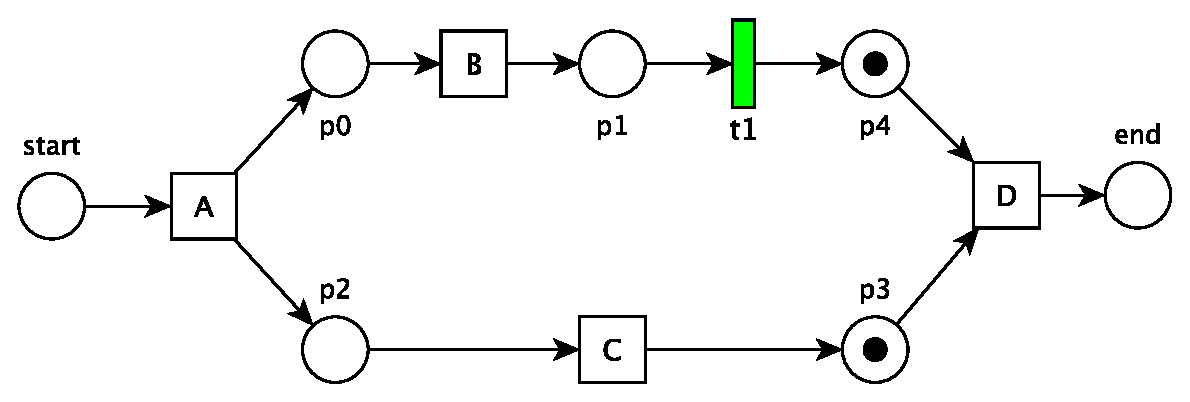
\includegraphics[scale=0.30]{./fig/LogReplay3e}
  \end{center}
  \begin {block}{Measures}
    \begin{tabular}{cccccc}
                  & p0 & p2 & p1 & p3 & p4 \\
       $\TSync$   & 0  & 0  & 0  & 4  & 0  \\
       $\TTot$    & 1  & 3  & 6  &    &   \\
    \end{tabular}
  \end{block}
}
\frame{
  \begin{block}{Log-replay examples}
    Trace log $(A, 1s), (B, 2s), (C, 4), \alert{(D, 8s)}$ 
  \end{block}
  \begin{center}
    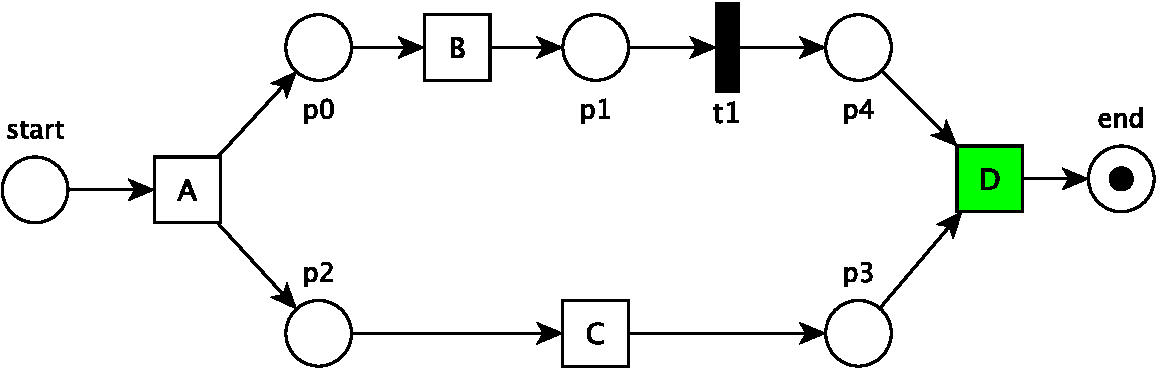
\includegraphics[scale=0.30]{./fig/LogReplay3f}
  \end{center}
  \begin {block}{Measures}
    \begin{tabular}{cccccc}
                  & p0 & p2 & p1 & p3 & p4 \\
       $\TSync$   & 0  & 0  & 0  & 4  & 0  \\
       $\TTot$    & 1  & 3  & 6  & 4  & 0 \\
    \end{tabular}
  \end{block}
}

%%% Local Variables: 
%%% mode: latex
%%% TeX-master: "main"
%%% End: 


  %   \subsection{Analisi di Performance}
  %   \frame{
  %     \begin{block}{Analisi di Performance}
  %       \begin{itemize}
  % 	\item L'idea è di calcolare l'intervallo di tempo tra produzione e consumo di token in ogni piazza della rete. 
  % 	\item Fruttando il log-replay si possono calcolare le metriche di performance.
  %   
  %   \begin{itemize}
  %       \item Si parte dall'algoritmo standard di log replay che produce la lista delle transizioni
  % 	  \item Si trasforma la lista di transizioni in una sequenza \textquotedblleft eager\textquotedblright
  %       $R = [tr_1, .... , tr_n]$ per ogni $tr_i$  transizione invisibile
  %       \begin{itemize}
  % 	\item Sia $tr_p$ l'ultima ($p < i$) transizione visibile
  % 	\item $\bullet tr_i \cap tr_p \bullet  \not = \emptyset$
  %       \end{itemize}
  %       
  %       \item Per ogni transizione invisibile $tr_i$
  % 	
  % 	\begin{enumerate}
  % 	  \item sposto a sinistra la transizione fino a quando non trovo una transizione visibile $\bullet tr_i \cap tr_p \bullet  \not =
  % 	    \emptyset$ 
  % 	\end{enumerate}
  % 	
  % \end{itemize}
  %     
  %       \end{itemize}
  % 
  %     \end{block}
  % 
  %   }

    \frame{
  \begin{block}{Esempio Calcolo Performance}
    
    \begin{itemize}
      \item Eventi del log $(A, 1s), (B, 2s), (C, 4), (D, 8s)$ 
      \item Sequenza di transizioni del log replay  $A, B, C, t1, D$
      \item Risultato della sequenza \textquotedblleft eager\textquotedblright $A, B, t1, C, D$
    \end{itemize}

  \end{block}
  \begin{center}
    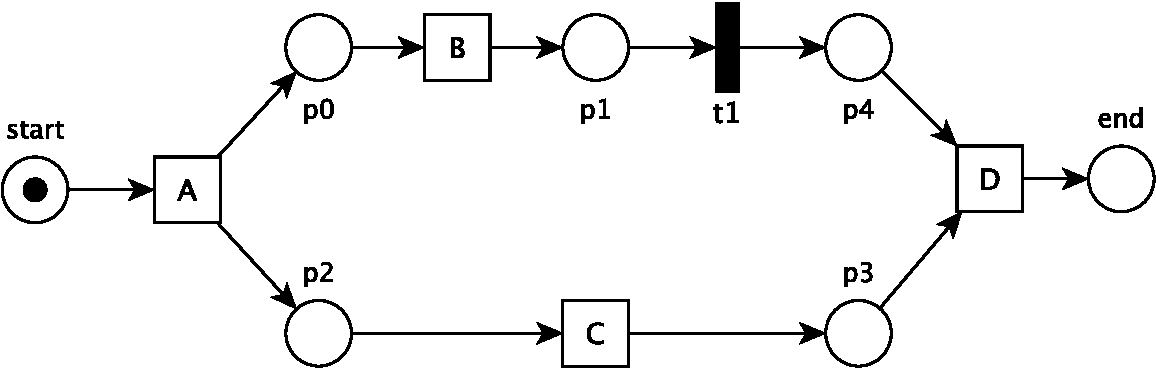
\includegraphics[scale=0.30]{./fig/LogReplay3a}
  \end{center}
  \begin {block}{Misure}
    \begin{tabular}{ccc}
                  \\
       $\TSync$   \\
       $\TTot$    \\
    \end{tabular}
  \end{block}
}

\frame{
  \begin{block}{Esempio Calcolo Performance}
    
    \begin{itemize}
      \item Eventi del log $\alert{(A, 1s)}, (B, 2s), (C, 4), (D, 8s)$ 
      \item Sequenza di transizioni del log replay  $A, B, C, t1, D$
      \item Risultato della sequenza \textquotedblleft eager\textquotedblright $\alert{A}, B, t1, C, D$
    \end{itemize}

  \end{block}
  \begin{center}
    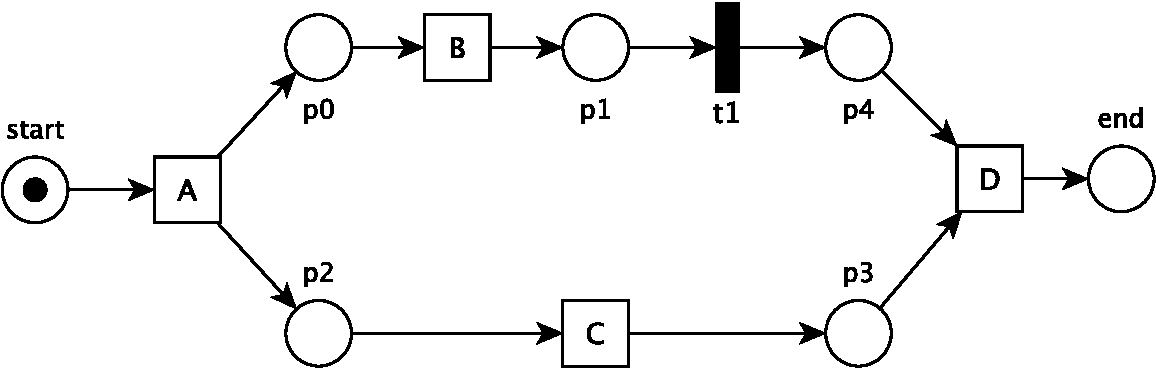
\includegraphics[scale=0.30]{./fig/LogReplay3a}
  \end{center}
  \begin {block}{Misure}
    \begin{tabular}{ccc}
                  \\
       $\TSync$   \\
       $\TTot$    \\
    \end{tabular}
  \end{block}
}

\frame{
  \begin{block}{Esempio Calcolo Performance}
    
    \begin{itemize}
      \item Eventi del log $\alert{(A, 1s)}, (B, 2s), (C, 4), (D, 8s)$ 
      \item Sequenza di transizioni del log replay  $A, B, C, t1, D$
      \item Risultato della sequenza \textquotedblleft eager\textquotedblright $\alert{A}, B, t1, C, D$
    \end{itemize}

  \end{block}
  \begin{center}
    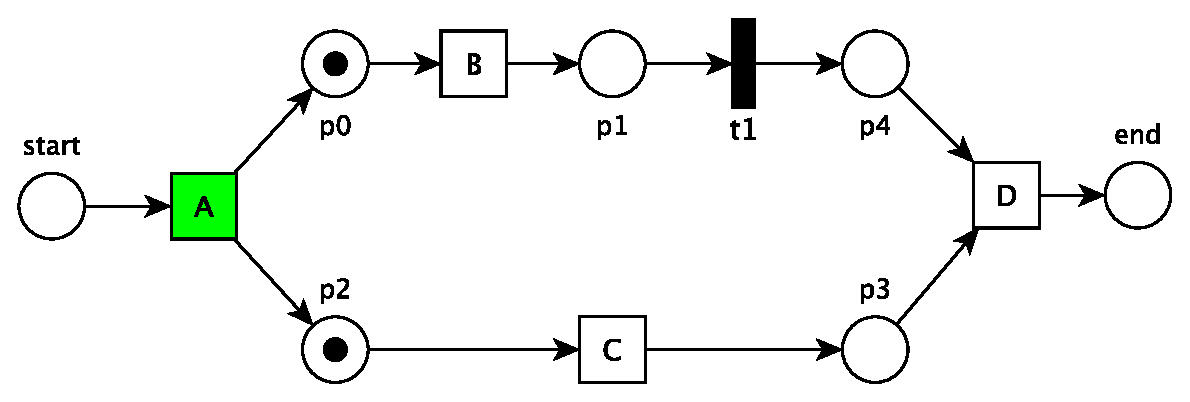
\includegraphics[scale=0.30]{./fig/LogReplay3b}
  \end{center}
  \begin {block}{Misure}
    \begin{tabular}{ccc}
                  & p0 & p2 \\
       $\TSync$   & 0  & 0  \\
       $\TTot$    &    &    \\
    \end{tabular}
  \end{block}
}
\frame{
  \begin{block}{Esempio Calcolo Performance}
    
    \begin{itemize}
      \item Eventi del log $(A, 1s), \alert{(B, 2s)}, (C, 4), (D, 8s)$ 
      \item Sequenza di transizioni del log replay  $A, B, C, t1, D$
      \item Risultato della sequenza \textquotedblleft eager\textquotedblright $A, \alert{B}, t1, C, D$
    \end{itemize}

  \end{block}
  \begin{center}
    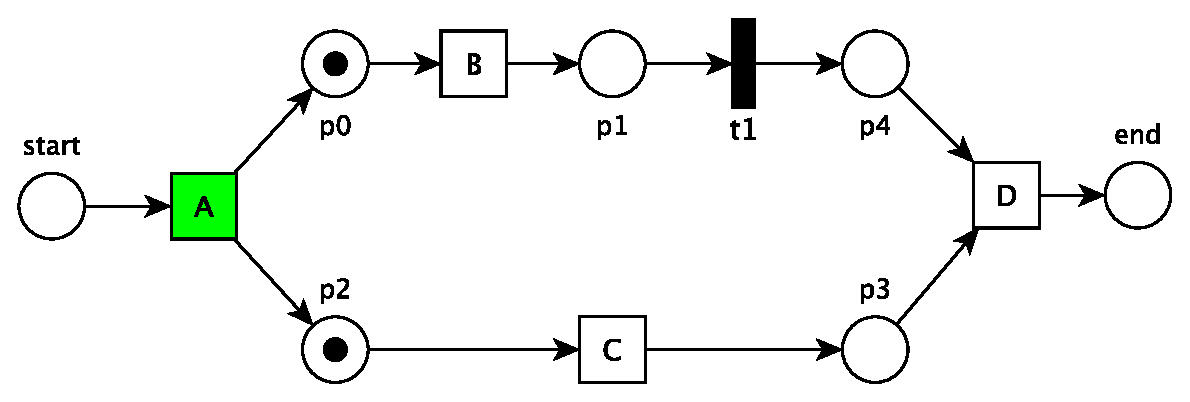
\includegraphics[scale=0.30]{./fig/LogReplay3b}
  \end{center}
  \begin {block}{Misure}
    \begin{tabular}{ccc}
                  & p0 & p2 \\
       $\TSync$   & 0  & 0  \\
       $\TTot$    &    &    \\
    \end{tabular}
  \end{block}
}
\frame{
  \begin{block}{Esempio Calcolo Performance}
    
    \begin{itemize}
      \item Eventi del log $(A, 1s), \alert{(B, 2s)}, (C, 4), (D, 8s)$ 
      \item Sequenza di transizioni del log replay  $A, B, C, t1, D$
      \item Risultato della sequenza \textquotedblleft eager\textquotedblright $A, \alert{B}, t1, C, D$
    \end{itemize}

  \end{block}
  \begin{center}
    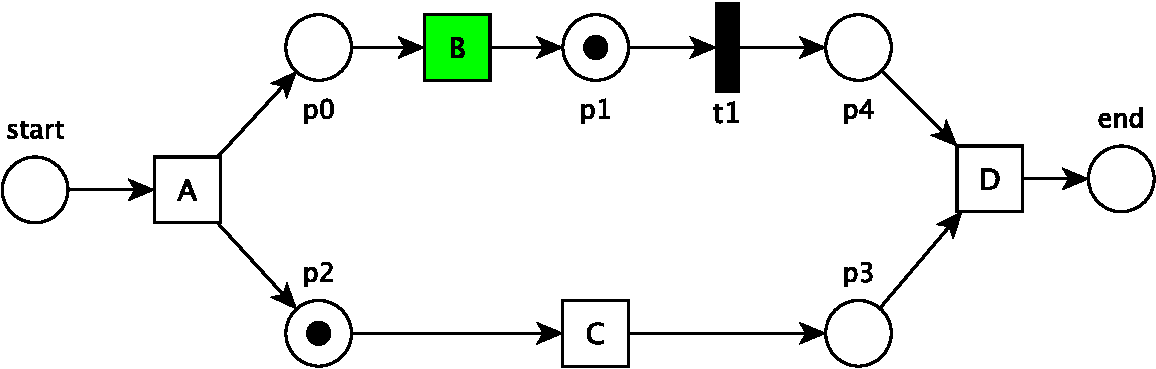
\includegraphics[scale=0.30]{./fig/LogReplay3c}
  \end{center}
  \begin {block}{Misure}
    \begin{tabular}{cccccc}
                  & p0 & p2 & p1 \\
       $\TSync$   & 0  & 0  & 0  \\
       $\TTot$    & 1  &    &    \\
    \end{tabular}
  \end{block}
}

% Attivazione di t1
\frame{
  \begin{block}{Esempio Calcolo Performance}
    
    \begin{itemize}
      \item Eventi del log $(A, 1s), \alert{(B, 2s)}, (C, 4), (D, 8s)$ 
      \item Sequenza di transizioni del log replay  $A, B, C, t1, D$
      \item Risultato della sequenza \textquotedblleft eager\textquotedblright $A, B, \alert{t1}, C, D$
    \end{itemize}

  \end{block}
  \begin{center}
    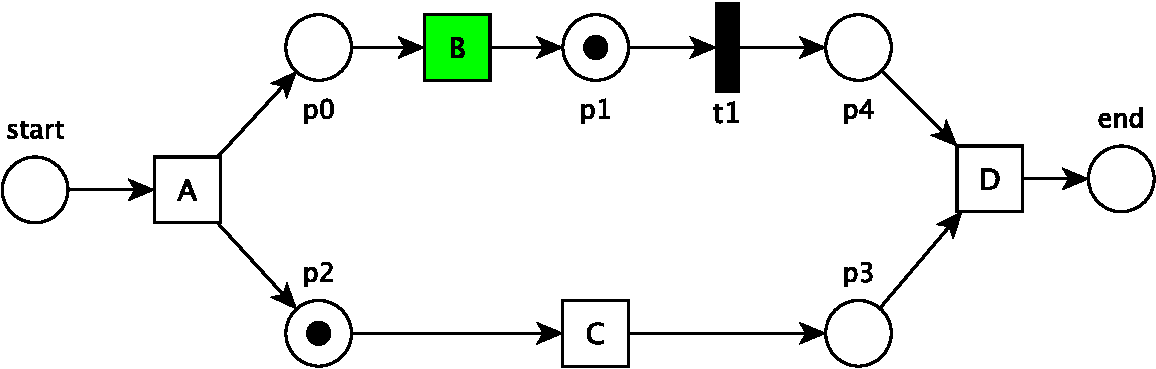
\includegraphics[scale=0.30]{./fig/LogReplay3c}
  \end{center}
  \begin {block}{Misure}
    \begin{tabular}{cccccc}
                  & p0 & p2 & p1 \\
       $\TSync$   & 0  & 0  & 0  \\
       $\TTot$    & 1  &    &    \\
    \end{tabular}
  \end{block}
}
\frame{
  \begin{block}{Esempio Calcolo Performance}
    
    \begin{itemize}
      \item Eventi del log $(A, 1s), \alert{(B, 2s)}, (C, 4), (D, 8s)$ 
      \item Sequenza di transizioni del log replay  $A, B, C, t1, D$
      \item Risultato della sequenza \textquotedblleft eager\textquotedblright $A, B, \alert{t1}, C, D$
    \end{itemize}
  \end {block}
  \begin{center}
    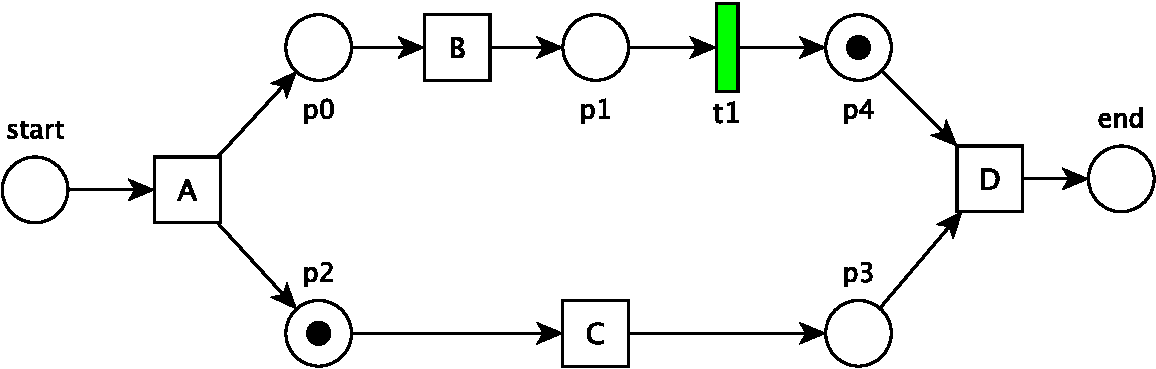
\includegraphics[scale=0.30]{./fig/LogReplay4d}
  \end{center}
  \begin {block}{Misure}
    \begin{tabular}{cccccc}
                  & p0 & p2 & p1 & p3 & p4 \\
       $\TSync$   & 0  & 0  & 0  &    &    \\
       $\TTot$    & 1  &    & 0  &    &    \\
    \end{tabular}
  \end{block}
}

\frame{
  \begin{block}{Esempio Calcolo Performance}
    
    \begin{itemize}
      \item Eventi del log $(A, 1s), (B, 2s), \alert{(C, 4)}, (D, 8s)$ 
      \item Sequenza di transizioni del log replay  $A, B, C, t1, D$
      \item Risultato della sequenza \textquotedblleft eager\textquotedblright $A, B, t1, \alert{C}, D$
    \end{itemize}
  \end {block}
  \begin{center}
    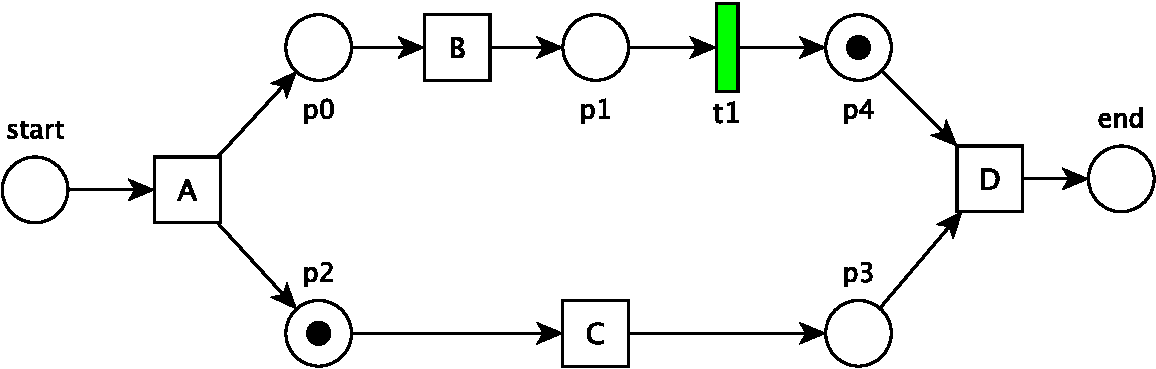
\includegraphics[scale=0.30]{./fig/LogReplay4d}
  \end{center}
  \begin {block}{Misure}
    \begin{tabular}{cccccc}
                  & p0 & p2 & p1 & p3 & p4 \\
       $\TSync$   & 0  & 0  & 0  &    &    \\
       $\TTot$    & 1  &    & 0  &    &    \\
    \end{tabular}
  \end{block}
}
\frame{
  \begin{block}{Esempio Calcolo Performance}
    
    \begin{itemize}
      \item Eventi del log $(A, 1s), (B, 2s), \alert{(C, 4)}, (D, 8s)$ 
      \item Sequenza di transizioni del log replay  $A, B, C, t1, D$
      \item Risultato della sequenza \textquotedblleft eager\textquotedblright $A, B, t1, \alert{C}, D$
    \end{itemize}
  \end {block}
  \begin{center}
    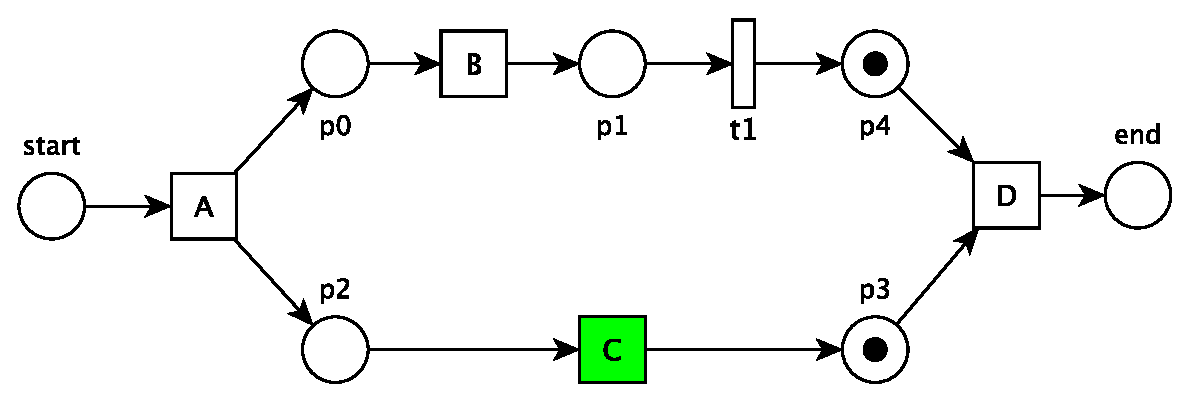
\includegraphics[scale=0.30]{./fig/LogReplay4e}
  \end{center}
  \begin {block}{Misure}
    \begin{tabular}{cccccc}
                  & p0 & p2 & p1 & p3 & p4 \\
       $\TSync$   & 0  & 0  & 0  & 0  & 2  \\
       $\TTot$    & 1  & 2  & 0  &    &    \\
    \end{tabular}
  \end{block}
}
\frame{
  \begin{block}{Esempio Calcolo Performance}
    
    \begin{itemize}
      \item Eventi del log $(A, 1s), (B, 2s), (C, 4), \alert{(D, 8s)}$ 
      \item Sequenza di transizioni del log replay  $A, B, C, t1, D$
      \item Risultato della sequenza \textquotedblleft eager\textquotedblright $A, B, t1, C, \alert{D}$
    \end{itemize}
  \end {block}
  \begin{center}
    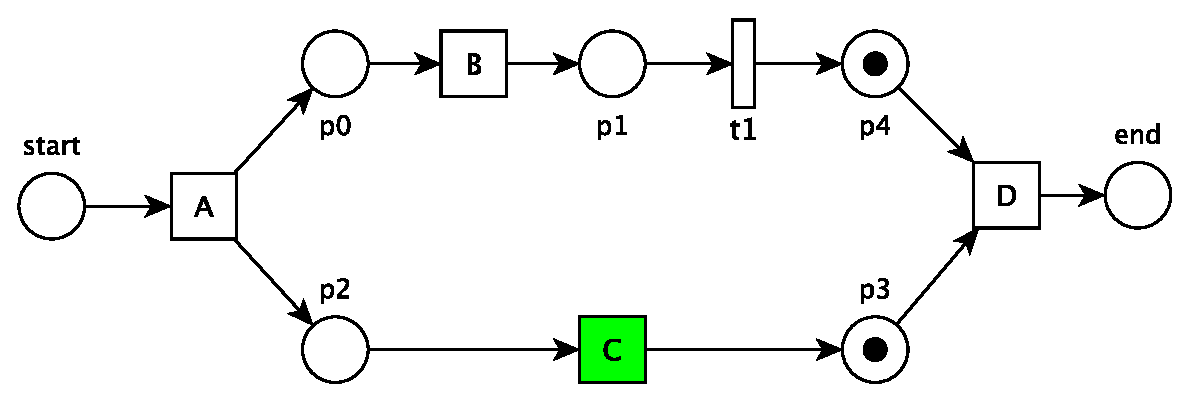
\includegraphics[scale=0.30]{./fig/LogReplay4e}
  \end{center}
  \begin {block}{Misure}
    \begin{tabular}{cccccc}
                  & p0 & p2 & p1 & p3 & p4 \\
       $\TSync$   & 0  & 0  & 0  & 0  & 2  \\
       $\TTot$    & 1  & 2  & 0  &   &   \\
    \end{tabular}
  \end{block}
}
\frame{
  \begin{block}{Esempio Calcolo Performance}
    
    \begin{itemize}
      \item Eventi del log $(A, 1s), (B, 2s), (C, 4), \alert{(D, 8s)}$ 
      \item Sequenza di transizioni del log replay  $A, B, C, t1, D$
      \item Risultato della sequenza \textquotedblleft eager\textquotedblright $A, B, t1, C, \alert{D}$
    \end{itemize}
  \end {block}
  \begin{center}
    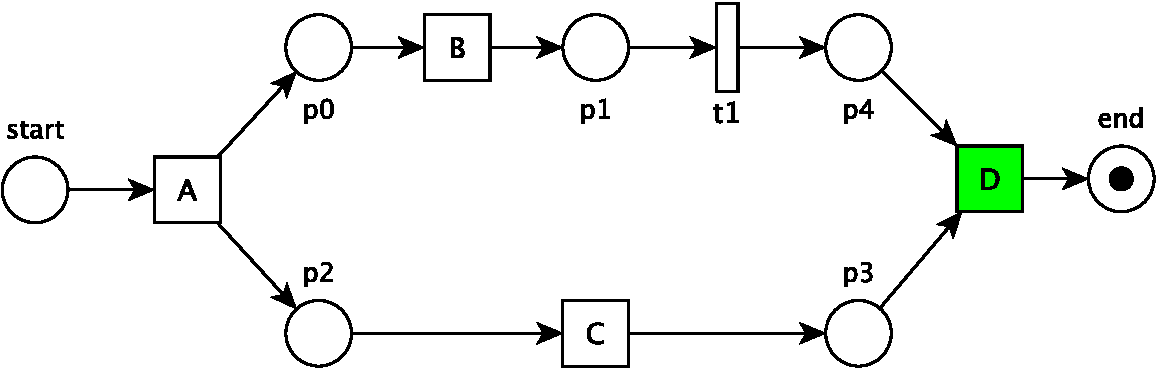
\includegraphics[scale=0.30]{./fig/LogReplay4f}
  \end{center}
  \begin {block}{Misure}
    \begin{tabular}{cccccc}
                  & p0 & p2 & p1 & p3 & p4 \\
       $\TSync$   & 0  & 0  & 0  & 0  & 2  \\
       $\TTot$    & 1  & 2  & 0  & 4  & 6  \\
    \end{tabular}
  \end{block}
}
%%% Local Variables: 
%%% mode: latex
%%% TeX-master: "main"
%%% End: 


  \section{Proiezioni dei dati sul modello}
    \subsection{Dall'analisi al BPMN}
  

  %   \frame{
  %     \begin{block}{Dall'analisi al BPMN (Performance)}
  %       \begin{itemize}
  % 	\item \alert{Tempo di Attesa}: transizione invisibile è fired
  % 	  immediatamente $\Rightarrow$ nei place pre-set delle transizioni visibili
  % 	\item \alert{Tempo di Sincronizzazione} nei place che hanno almeno una transizione nel loro post-set che dipende da
  % un altro place.
  %       \end{itemize}
  %     \end{block}
  %     
  %     \begin{center}
  %       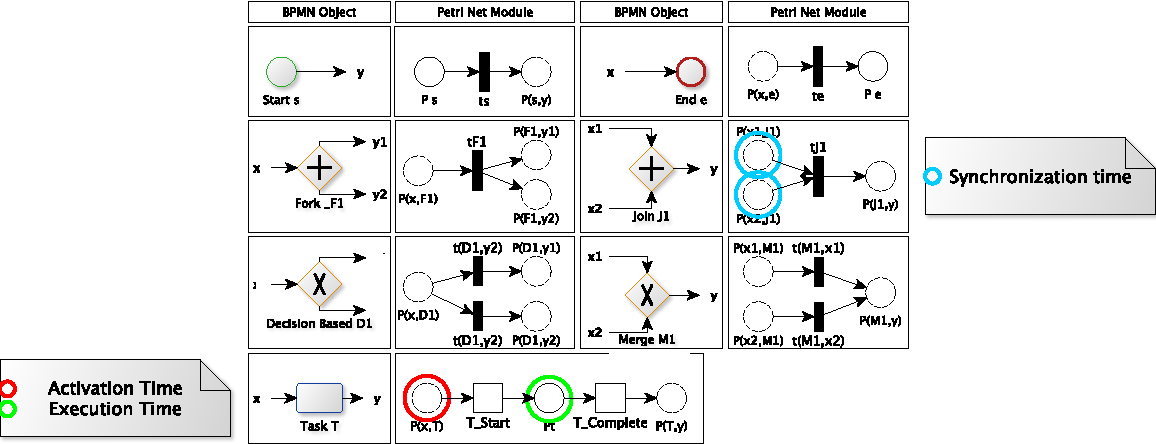
\includegraphics[scale=0.50]{./fig/MappingBPMNtoPN3}
  %     \end{center}
  % 
  %   }

    \frame{
    \begin{block}{Dall'analisi al BPMN (Performance)}
	\begin{itemize}
	  \item \alert{Tempi di Attesa}: sono nei place pre-set delle transizioni visibili
	  \item \alert{Tempi di Sincronizzazione}: sono nei place che hanno almeno una transizione nel loro post-set che dipende da
  un altro place.
	\end{itemize}
      \end{block}

      
	\begin{center}
	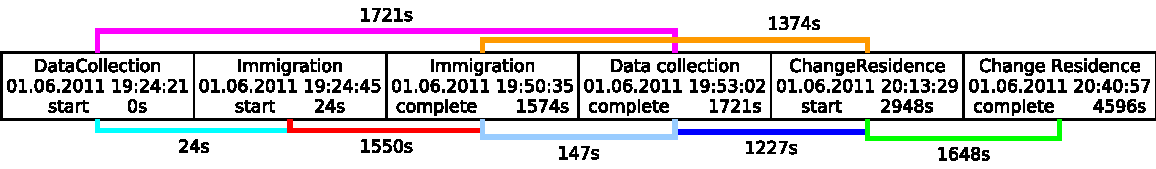
\includegraphics[scale=0.35]{./fig/Log} \\
	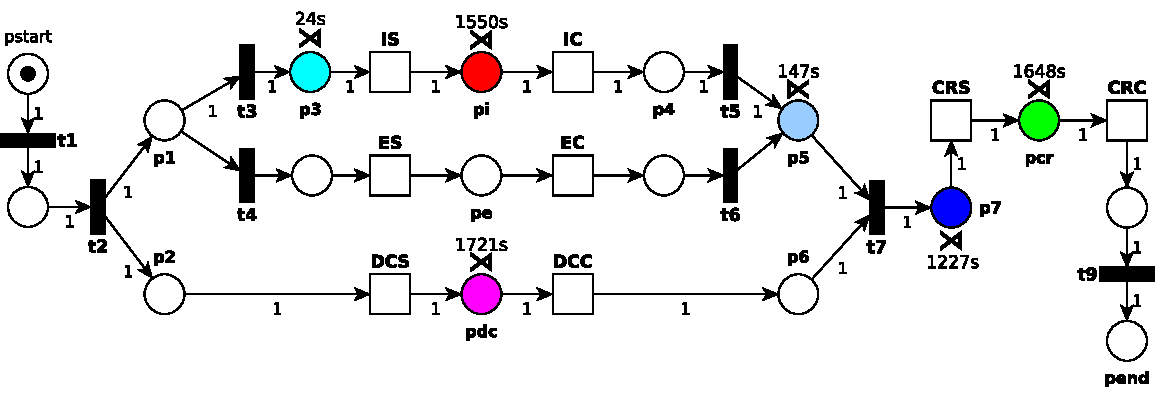
\includegraphics[scale=0.35]{./fig/PerformanceProM6PatchConAnnotazioni} \\
	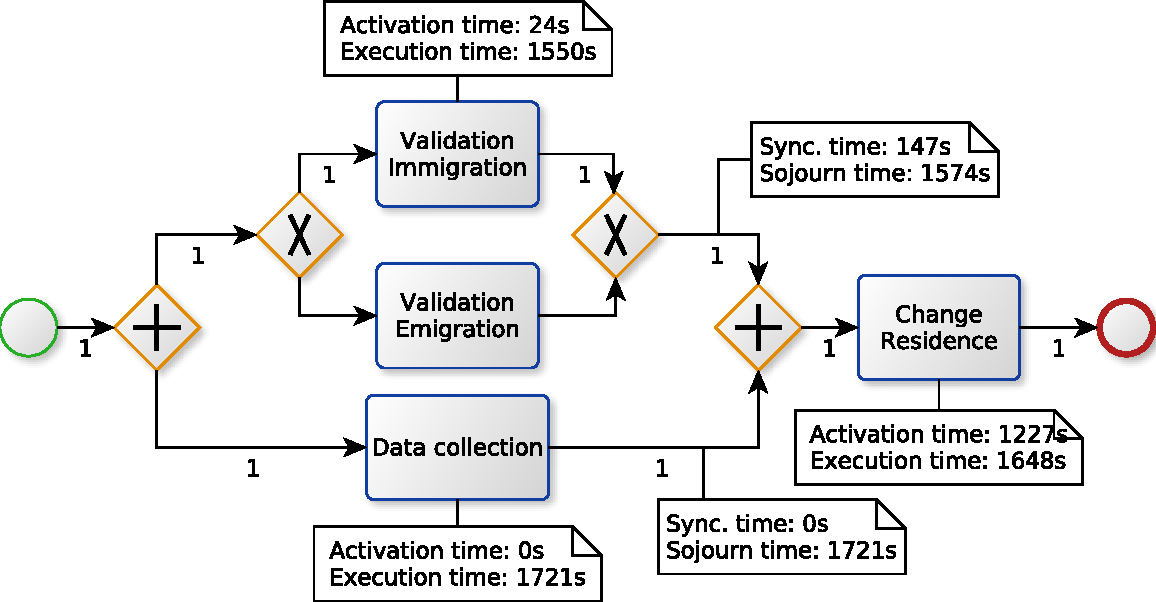
\includegraphics[scale=0.25]{./fig/residencyHiLevel}
      \end{center}
      
      
      

    }

  %  \frame{
  %     \begin{block}{Dall'analisi al BPMN (Conformance)}
  %       \begin{itemize}
  % 	\item \alert{Missing tokens}: Log replay produce missing tokens solo per il fire
  % 	  delle transizioni visibili $\Rightarrow$ pre-set di una transizione visibile
  % 	\item \alert{Remaining tokens} Le transizioni invisibili sono fired solo se richiesto da una successiva
  % transizione visibile  $\Rightarrow$ nei place  post-set di una transizione visibile o di una transizione
  % invisibile che generano più di un token.
  % 
  %       \end{itemize}
  %     \end{block}
  %     
  %     \begin{center}
  %       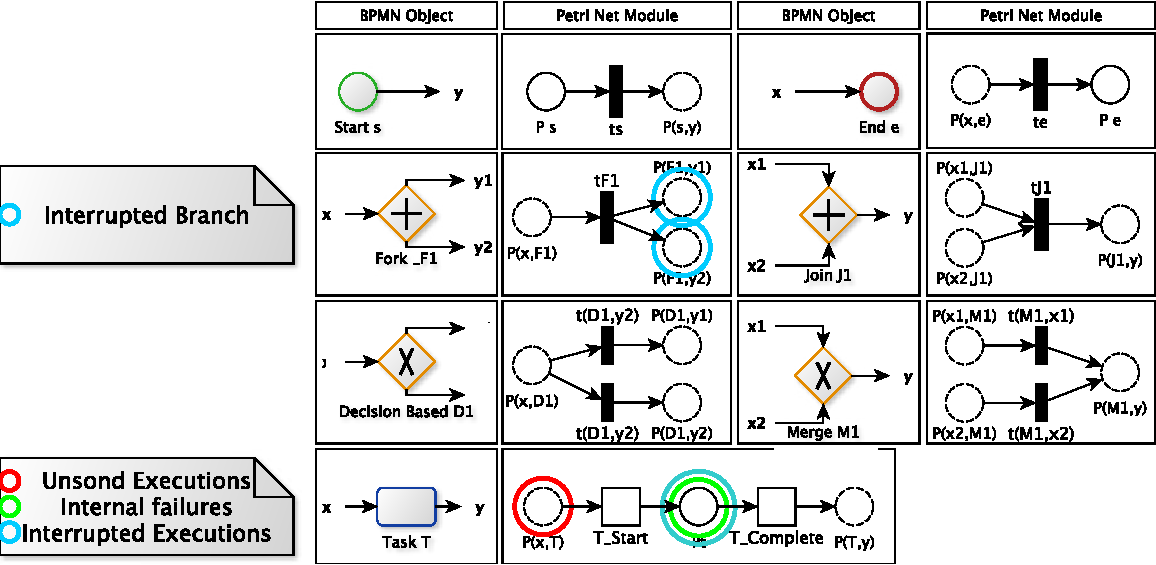
\includegraphics[scale=0.40]{./fig/MappingBPMNtoPN2}
  %     \end{center}
  % 
  %   }
    \frame{
      \begin{block}{Dall'analisi al BPMN (Conformance)}
	\begin{itemize}
	  \item \alert{Missing tokens}: nei place pre-set di una transizione visibile
	  \item \alert{Remaining tokens}  nei place post-set di una transizione visibile o di una transizione
  invisibile che generano più di un token.
	\end{itemize}
      \end{block}
  
      
	\begin{center}
	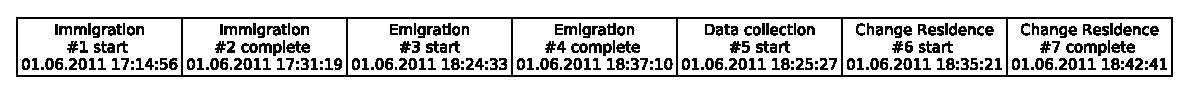
\includegraphics[scale=0.45]{./fig/LogConformance} \\ 
	\includegraphics[scale=0.45]{./fig/residencyPNConformance} \\  
	\includegraphics[scale=0.3]{./fig/residencyHiLevelConformace}    
      \end{center}
      
      
    

    }

    \section{Conclusioni}
    \frame{
      \begin{block}{Risultati teorici}
	
	\begin{itemize}
	  \item Affinate le tecniche per gestire le transizioni invisibili sulle Petri Net
	  \item Proiezioni delle misure sul BPMN
	\end{itemize}

      \end{block}
      \begin{block}{Risultati di sviluppo}
	
	\begin{itemize}
      
	\item Nuovi plug-ins per ProM
	  \begin{itemize}
	    \item Transformazione del modello BPMN in una Petri Net
	    \item Analisi di Performance e Conformance su Petri Net 
	    \item Proiezioni delle misure di analisi sul modello BPMN di partenza.
	  \end{itemize}
	\end{itemize}

      \end{block}
    }
    \frame{\tableofcontents}

    \end{document}


    %%% Local Variables: 
    %%% mode: latex
    %%% TeX-master: t
    %%% End: 
